\documentclass[11pt,a4paper]{article}
% Shared look for Laile's submission documents. Build with Tectonic (see submission/build.sh).
\usepackage{fontspec}
\usepackage{xcolor}
\usepackage{graphicx}
\usepackage{tikz}
\usetikzlibrary{positioning,fit,backgrounds,arrows.meta,calc,shapes.misc}

% macOS system fonts: Avenir Next for text, Hiragino Sans GB for 莱乐.
\setmainfont{Avenir Next.ttc}[
  Path=/System/Library/Fonts/,
  UprightFeatures={FontIndex=7},
  BoldFont={Avenir Next.ttc}, BoldFeatures={FontIndex=2},
  ItalicFont={Avenir Next.ttc}, ItalicFeatures={FontIndex=4},
  BoldItalicFont={Avenir Next.ttc}, BoldItalicFeatures={FontIndex=3}]
\setsansfont{Avenir Next.ttc}[
  Path=/System/Library/Fonts/,
  UprightFeatures={FontIndex=7},
  BoldFont={Avenir Next.ttc}, BoldFeatures={FontIndex=2},
  ItalicFont={Avenir Next.ttc}, ItalicFeatures={FontIndex=4},
  BoldItalicFont={Avenir Next.ttc}, BoldItalicFeatures={FontIndex=3}]
\newfontfamily\heavyfont{Avenir Next.ttc}[Path=/System/Library/Fonts/, UprightFeatures={FontIndex=8}]
\newfontfamily\cjk{Hiragino Sans GB.ttc}[Path=/System/Library/Fonts/, UprightFeatures={FontIndex=2}]

% The app's palette (DesignSystem/Theme.swift).
\definecolor{accent}{HTML}{0F8A6A}
\definecolor{accentsoft}{HTML}{DFF3EC}
\definecolor{reward}{HTML}{E8930C}
\definecolor{rewardsoft}{HTML}{FFF1DC}
\definecolor{danger}{HTML}{C62828}
\definecolor{dangersoft}{HTML}{FDE7E5}
\definecolor{ink}{HTML}{17211C}
\definecolor{muted}{HTML}{5D6B63}
\definecolor{surface}{HTML}{EEF2EF}
\definecolor{paper}{HTML}{F6F7F5}

\newcommand{\laile}{Laile ({\cjk 莱乐})}
\newcommand{\lele}{Lele ({\cjk 乐乐})}
\newcommand{\wordmark}{{\cjk\color{accent}莱乐}}

\usepackage[a4paper,margin=2.1cm,top=2cm,bottom=2.2cm]{geometry}
\usepackage[hidelinks]{hyperref}
\usepackage{enumitem}
\usepackage{booktabs}
\usepackage{tabularx}
\usepackage{caption}
\usepackage{titlesec}
\usepackage{fancyhdr}
\setlength{\fboxsep}{0pt}\setlength{\fboxrule}{0.4pt}

\setlength{\parindent}{0pt}
\newcolumntype{L}[1]{>{\raggedright\arraybackslash}p{#1}}
\newcolumntype{Y}{>{\raggedright\arraybackslash}X}
\setlength{\parskip}{6pt}
\linespread{1.08}
\setlist{nosep, leftmargin=1.2em, topsep=2pt}
\captionsetup{font={small,color=muted}, labelfont=bf, skip=4pt}
\titleformat{\section}{\Large\bfseries\color{accent}}{}{0pt}{}
\titleformat{\subsection}{\large\bfseries\color{ink}}{}{0pt}{}
\titlespacing*{\section}{0pt}{14pt}{4pt}
\titlespacing*{\subsection}{0pt}{10pt}{2pt}
\pagestyle{fancy}
\fancyhf{}
\renewcommand{\headrulewidth}{0pt}
\fancyfoot[L]{\footnotesize\color{muted}\laile\ \ project description}
\fancyfoot[R]{\footnotesize\color{muted}\thepage}
\color{ink}

% Things only the team can supply. They print in red so they can't be missed.
\newcommand{\fillin}[1]{\colorbox{dangersoft}{\color{danger}\textbf{TO ADD:} #1}}
\newcommand{\fillinblock}[1]{\noindent\colorbox{dangersoft}{\parbox{\dimexpr\linewidth-2\fboxsep}{\color{danger}\textbf{TO ADD:} #1}}}
\newcommand{\adpurl}{\href{https://adp.tencentcloud.com/webim_exp/\#/chat/nZbZZz}{adp.tencentcloud.com/webim\_exp/\#/chat/nZbZZz}}

% Phone screenshots, side by side.
\newcommand{\shot}[2]{\begin{minipage}[t]{0.235\linewidth}\centering
  \includegraphics[width=\linewidth]{../screenshots/#1}\\[2pt]{\scriptsize\color{muted}#2}\end{minipage}}

\begin{document}

% ------------------------------------------------------------------- title
\begin{minipage}[c]{0.2\linewidth}
  
\includegraphics[height=2.1cm]{../brand/mark-transparent.png}
\end{minipage}%
\begin{minipage}[c]{0.8\linewidth}
  {\fontsize{26}{28}\selectfont\bfseries Laile}\\[4pt]
  {\large Home physio that counts every rep and checks in.}
\end{minipage}

\vspace{8pt}
{\small\color{muted}
Tencent Cloud AI CAN DO IT Hackathon Singapore 2026 \ \textbullet\ \ Healthcare track (NTU LKC Medicine)\\
Challenge Statement 2: AI Healthier Every Day, intelligent support for long-term self-care\\
Charles Andrew Lim (solo) \ \textbullet\ \ Source: \href{https://github.com/LimCharles/laile}{github.com/LimCharles/laile}\\
Try Lele on Tencent Cloud ADP: \adpurl\\
Clinician portal: \href{https://43-156-108-79.sslip.io/portal}{43-156-108-79.sslip.io/portal}, login \texttt{clinician@laile.demo} / \texttt{laile-demo-2026}\\
Web app, no install: \href{https://43-156-108-79.sslip.io/app}{43-156-108-79.sslip.io/app} (tap a demo account, no sign-in)\\
iPhone app on TestFlight: \href{https://testflight.apple.com/join/WuymKzUH}{testflight.apple.com/join/WuymKzUH} (tap a demo account, no sign-in)}

\vspace{6pt}
{\color{accent}\rule{\linewidth}{1.2pt}}

\section{In one paragraph}
Most of physical therapy happens at home, between visits, where nobody can see it. \laile\ is an iPhone app, a web app and a clinician portal built around one idea: every program is measured by the phone's camera, and a coach called \lele\ keeps the person going between visits. A physio gives the patient a code; Lele drafts the program and the physio signs it. The first session is a check-in that sets personal targets from what the person can comfortably do. During sessions the camera counts reps and measures joint angles while Lele talks the person through each move and listens for pain. Between sessions Lele checks in, reminds, notices when things stall, and remembers what was sore. When goals change, the person tells Lele in chat and Lele drafts a new program; a physio patient's plan goes to their physio to approve first. The physio sees all of it, live, with a daily list of what needs attention and a short brief Lele writes from the person's record. When physio ends, the person moves on to a calisthenics program with their limits carried over, so the habit outlasts the treatment.

\section{The problem}
Home exercise is where rehabilitation succeeds or fails, and it is hard to sustain.
\begin{itemize}
  \item \textbf{People stop.} Estimates of non-adherence to home exercise in rehabilitation run as high as 50\% \cite{argent2018}.
  \item \textbf{The reasons are known and human.} A systematic review of 20 studies in musculoskeletal outpatient physiotherapy found strong evidence linking poor adherence to low activity before treatment, low self-efficacy, low mood, anxiety, helplessness, poor social support, more perceived barriers to exercise and pain during exercise \cite{jack2010}.
  \item \textbf{What helps is also known.} Reviewed trials point to activity monitoring with feedback, written instructions, goal setting and booster sessions as promising \cite{peek2016}. A reminder and a checkbox reach none of the barriers above.
  \item \textbf{The physio is blind between visits.} Self-reported logs cannot show whether an exercise was done, done well, or stopped because it hurt. Problems surface weeks later at the next appointment.
  \item \textbf{The need is growing in Singapore.} In 2026, 21.4\% of Singapore citizens were aged 65 or older, above the United Nations threshold for a super-aged society \cite{nptd2026}. Joint replacements, stiff shoulders, falls prevention and staying strong enough to live independently all depend on exercise done at home.
\end{itemize}
The challenge statement asks for support that is empowering, personalised, longitudinal, safe, practical, strictly bounded and honest about uncertainty. Laile is designed against that list (section~\ref{sec:fit}).

\section{Who it is for}
\begin{tabularx}{\linewidth}{@{}L{3.4cm}Y@{}}
\toprule
\textbf{Mdm Tan, 68} & Two weeks after a knee replacement. Wants to climb the stairs to the temple. Her physio, Dr Nair, gave her a code. She does her program with Lele, tells it when something pinches, and takes her medicines when Lele reminds her. When she tells Lele she wants stairs to feel easier, Lele drafts a plan and sends it to Dr Nair.\\
\textbf{Mr Ong, 54} & Stiff right shoulder, diabetes. His arm lift is measured every session (95\textdegree\ to 128\textdegree\ over a month in the demo). He asked Dr Nair, through Lele, whether he could add a core program.\\
\textbf{Alex} & Desk job, no physio. Told Lele he wants a first pull-up and his back gets stiff from sitting. Lele built him a 20-minute plan and left out push-ups because his wrist clicks.\\
\textbf{Dr Nair, physio} & Sees a daily list of what Lele noticed, reads Lele's summary before a visit, watches sessions live, signs every program, approves extra programs and Lele's plans, and discharges patients to a follow-on program.\\
\bottomrule
\end{tabularx}

\section{What Laile does}

\subsection{Programs are the unit}
Everything a person does is a program: a physio's program joined with a code, a plan Lele builds from a short conversation about goals, or a calisthenics or mobility program from Laile's catalog. Only the physio can change or end a physio program. While a physio supervises someone, anything else they want to add goes to the physio as a request (Lele passes it on and tells them the answer).

\begin{center}
\shot{02-today.png}{Today: Lele's check-in and the signed program}\hfill
\shot{05-programs.png}{Programs: Lele's plan, catalog, physio code}\hfill
\shot{12-goals-conversation.png}{Goals in the person's own words}\hfill
\shot{13-plan-built.png}{Lele's plan, built from those goals}
\end{center}

\subsection{The first session is a check-in}
A program starts with a check-in. The person does each move once at a comfortable effort and taps ``That's enough''. The camera measures reps, holds and range, and Laile sets working targets at about 70\% of their best. A rep then counts at 90\% of the range they reached. In a physio program, targets are only ever made easier than the physio's dose. People redo the check-in every couple of weeks from Progress.

\subsection{Sessions: the camera counts, Lele coaches}
Apple Vision tracks the body on the phone. A deterministic session conductor counts reps that reach the target angle, times holds only while the person is in position, checks form, and checks the camera can see the joints it needs. Lele's voice takes turns like a conversation: it explains the move, says ``In your own time'', counts, and asks ``How did that feel?'' between sets. The person can speak at any moment (``it's pulling'', ``sharp pain'') or tap a reply. Fixed rules decide what happens: carry on, stop the set, stop the exercise, or end the session and get help. Precautions follow the person into every program, so a knee or wrist limit protects them in a squat class too.

\begin{center}
\shot{08-session.png}{Session: camera-counted heel slides}\hfill
\shot{09-targets-set.png}{Check-in result: targets set}\hfill
\shot{14-precautions-follow.png}{Precautions follow the person}\hfill
\shot{10-me-privacy.png}{Plain safety and privacy}
\end{center}

\subsection{Lele takes initiative, and you can talk back}
Lele runs a round several times a day. It asks a morning check-in while someone is in physio (``How's your knee compared with yesterday?''), reminds them about medicines at the times their doctor set, nudges once on a quiet day, asks what is getting in the way after a few missed days, notices plateaus, and helps them prepare questions before a visit. Every question comes with suggested replies, and people can also type or say their answer in their own words; Lele matches it to the option it means and keeps their words. Telling Lele ``it's quite swollen this morning'' makes that day's session gentler and tells the physio. Guardrails keep it from nagging: quiet hours from 9\,pm to 7\,am, at most three conversations started a day, and no repeats. The same reminders are scheduled as phone notifications so they arrive with the app closed.

\subsection{Lele remembers}
When something is sore during an exercise, Lele writes a care note with the exercise, the spot, how bad it was and the person's own words. Next time, that exercise is a little easier (a smaller bend counts as a full rep, or a shorter hold), and Lele says so. After two comfortable sessions it eases back a step at a time. The person and the physio see the same notes and history, and the physio can keep an exercise eased or add notes for Lele to follow.

\begin{center}
\shot{03-lele-inbox.png}{Lele's reminders and questions}\hfill
\shot{04-lele-chat.png}{Lele on ADP, using real numbers}\hfill
\shot{06-ask-physio.png}{Adding a program asks the physio}\hfill
\shot{07-today-program-meds.png}{Program and today's medicines}
\end{center}

\subsection{Plan with Lele in chat}
Goals change: a person wants stairs to feel easier, or a first push-up. They tap ``Plan a new program'' or simply tell Lele ``my goals have changed''. Lele asks five short questions (what to work on, minutes a day, experience, anything that hurts, and a safety check), each with suggested answers and open to their own words. Lele on Tencent Cloud ADP then drafts the program, using the knowledge base for what suits those goals and only exercises from Laile's vetted library; Laile's code checks the draft against the person's limits. Without a physio, the new plan replaces Lele's previous one and starts with a check-in. With a physio, nothing starts: the plan goes to the physio's daily list to approve, and Lele tells the person the answer. A safety answer like ``my doctor told me to be careful'' is saved to the person's notes, and someone recovering from an injury, or easing aches in a sore spot, is also encouraged to see a physio.

\subsection{What Lele knows about each person}
Every conversation and session adds to a record Lele reads before it answers: goals, minutes a day, experience, areas to go easy on, care notes (sore spots in the person's own words, what was eased and why, the physio's notes), measurements against baseline, adherence and open requests. The person sees it on their Me screen as ``What Lele knows about you'' and ``What Lele remembers''. The same record is what Lele summarises for the physio, so the person, the physio and Lele work from one set of facts.

\begin{figure}[htbp]
\centering
\fbox{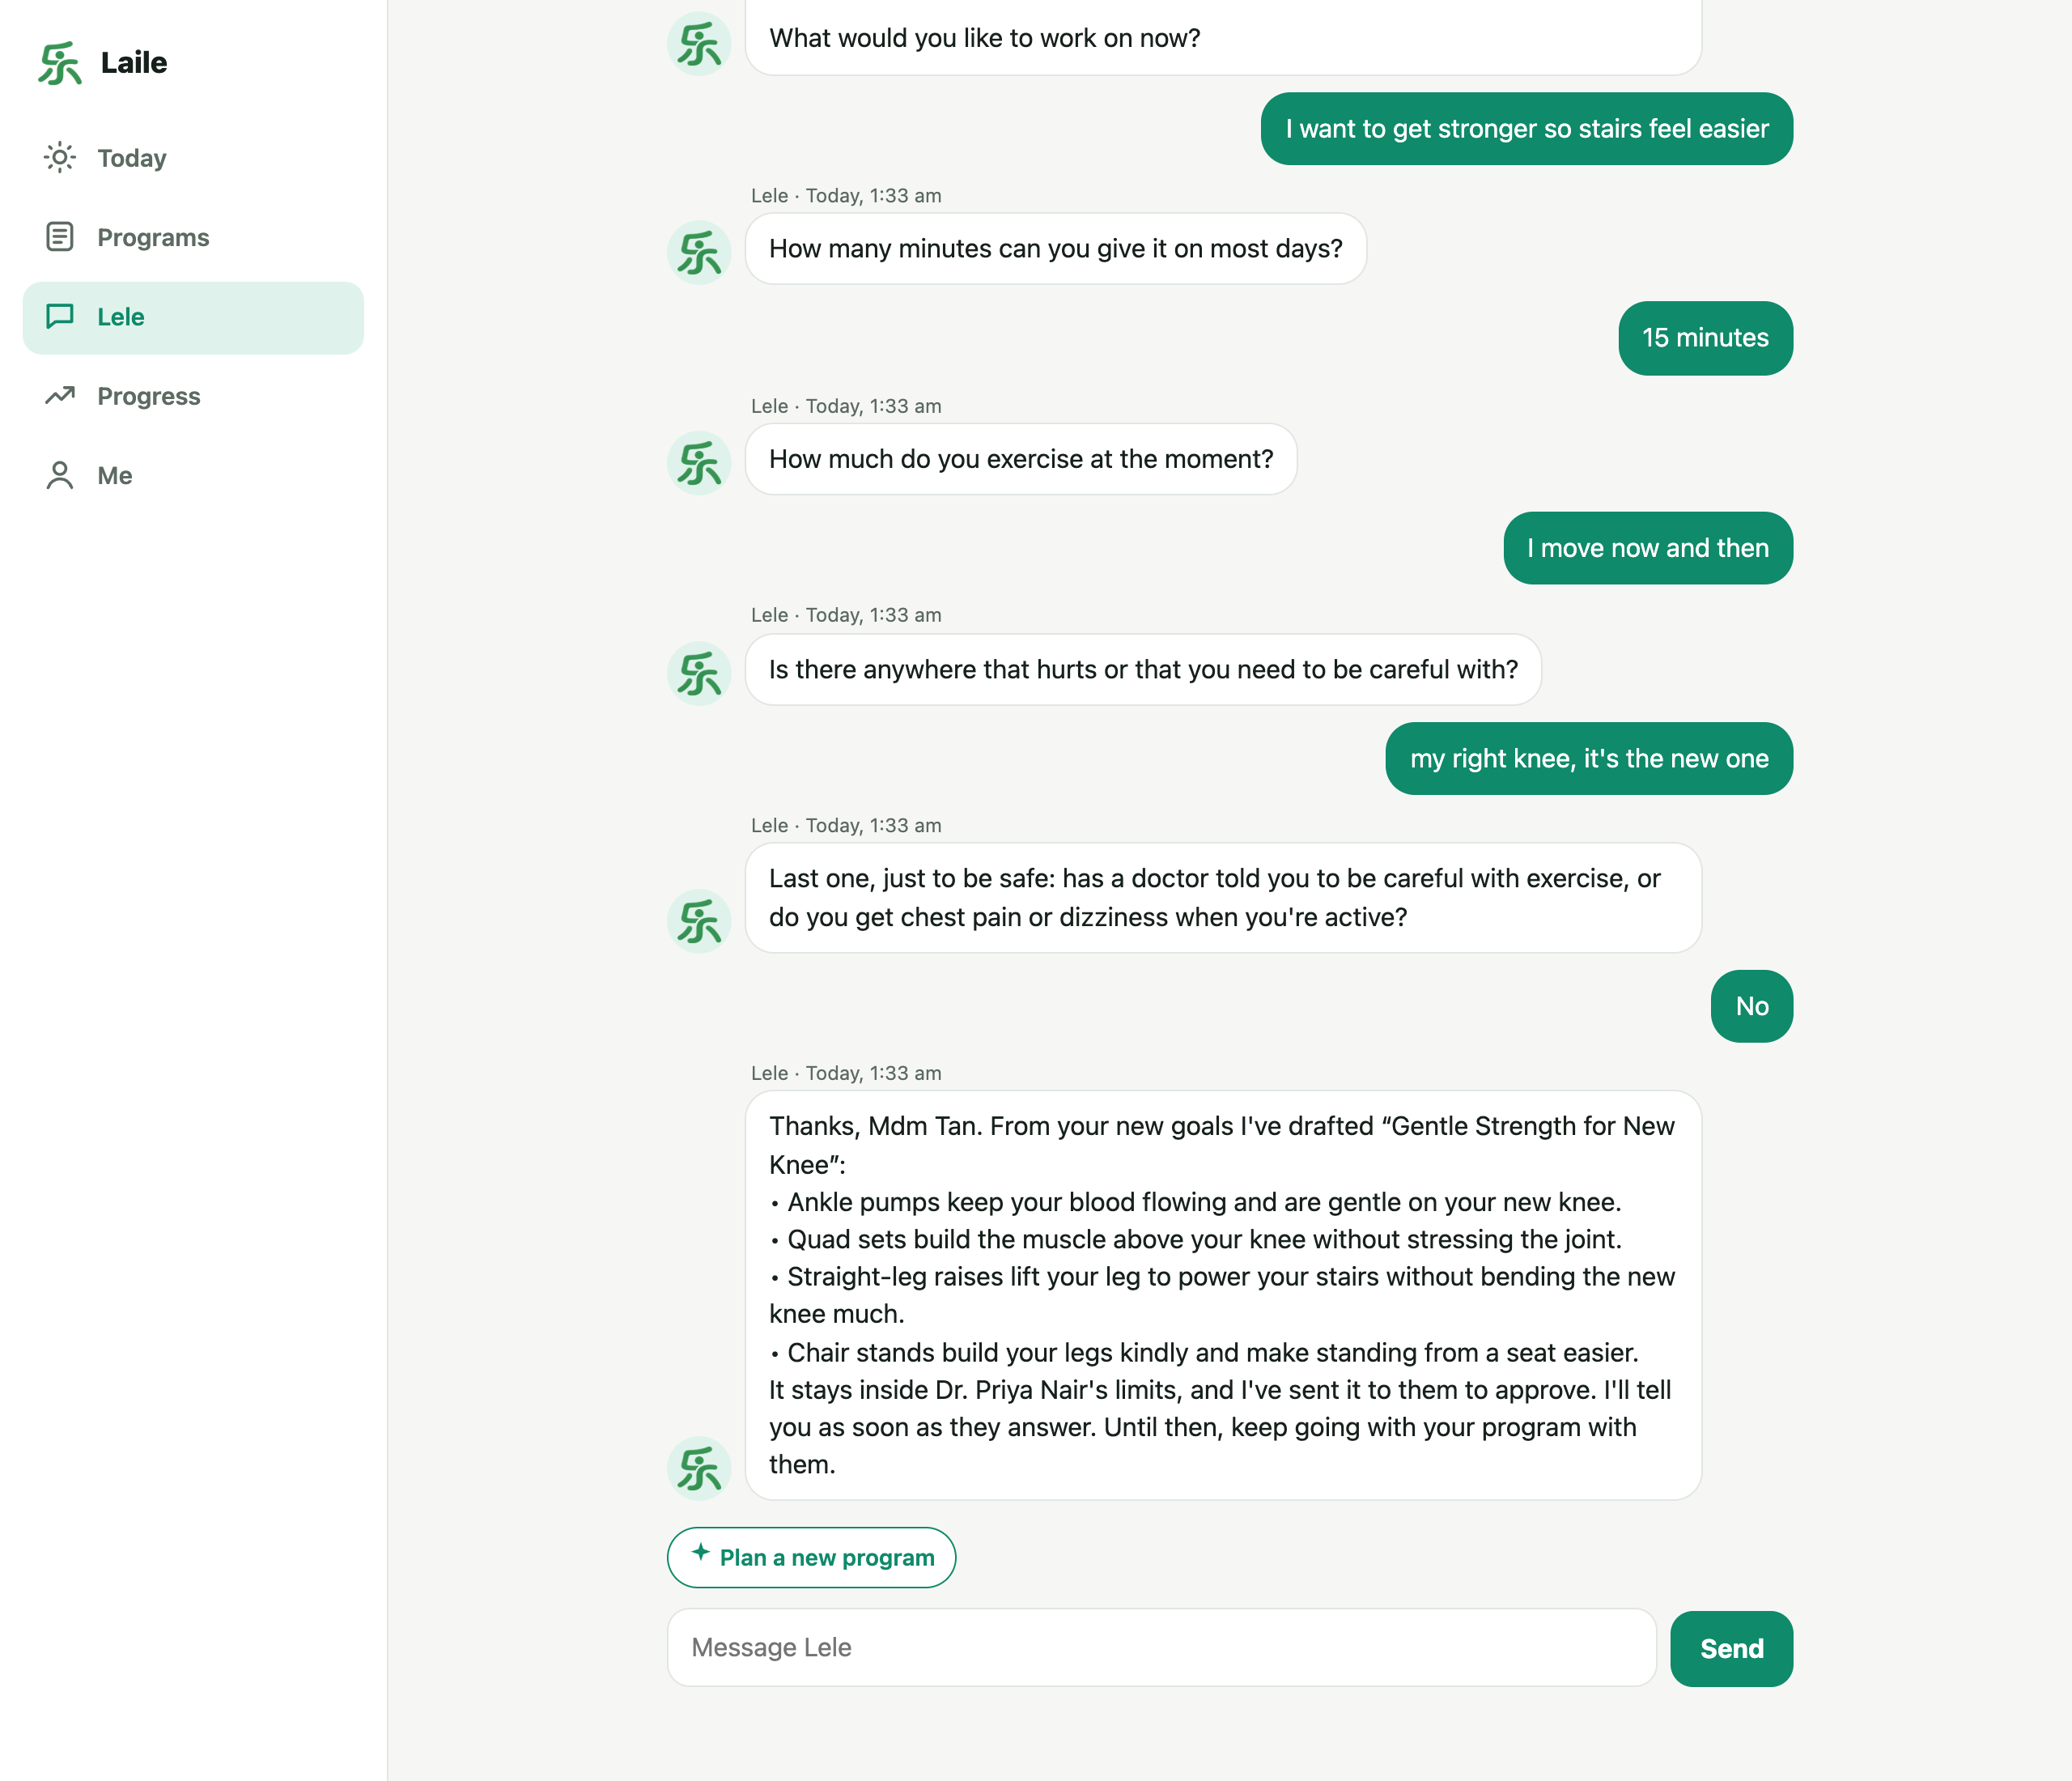
\includegraphics[width=0.49\linewidth]{../screenshots/31-web-lele-plan.png}}\hfill
\fbox{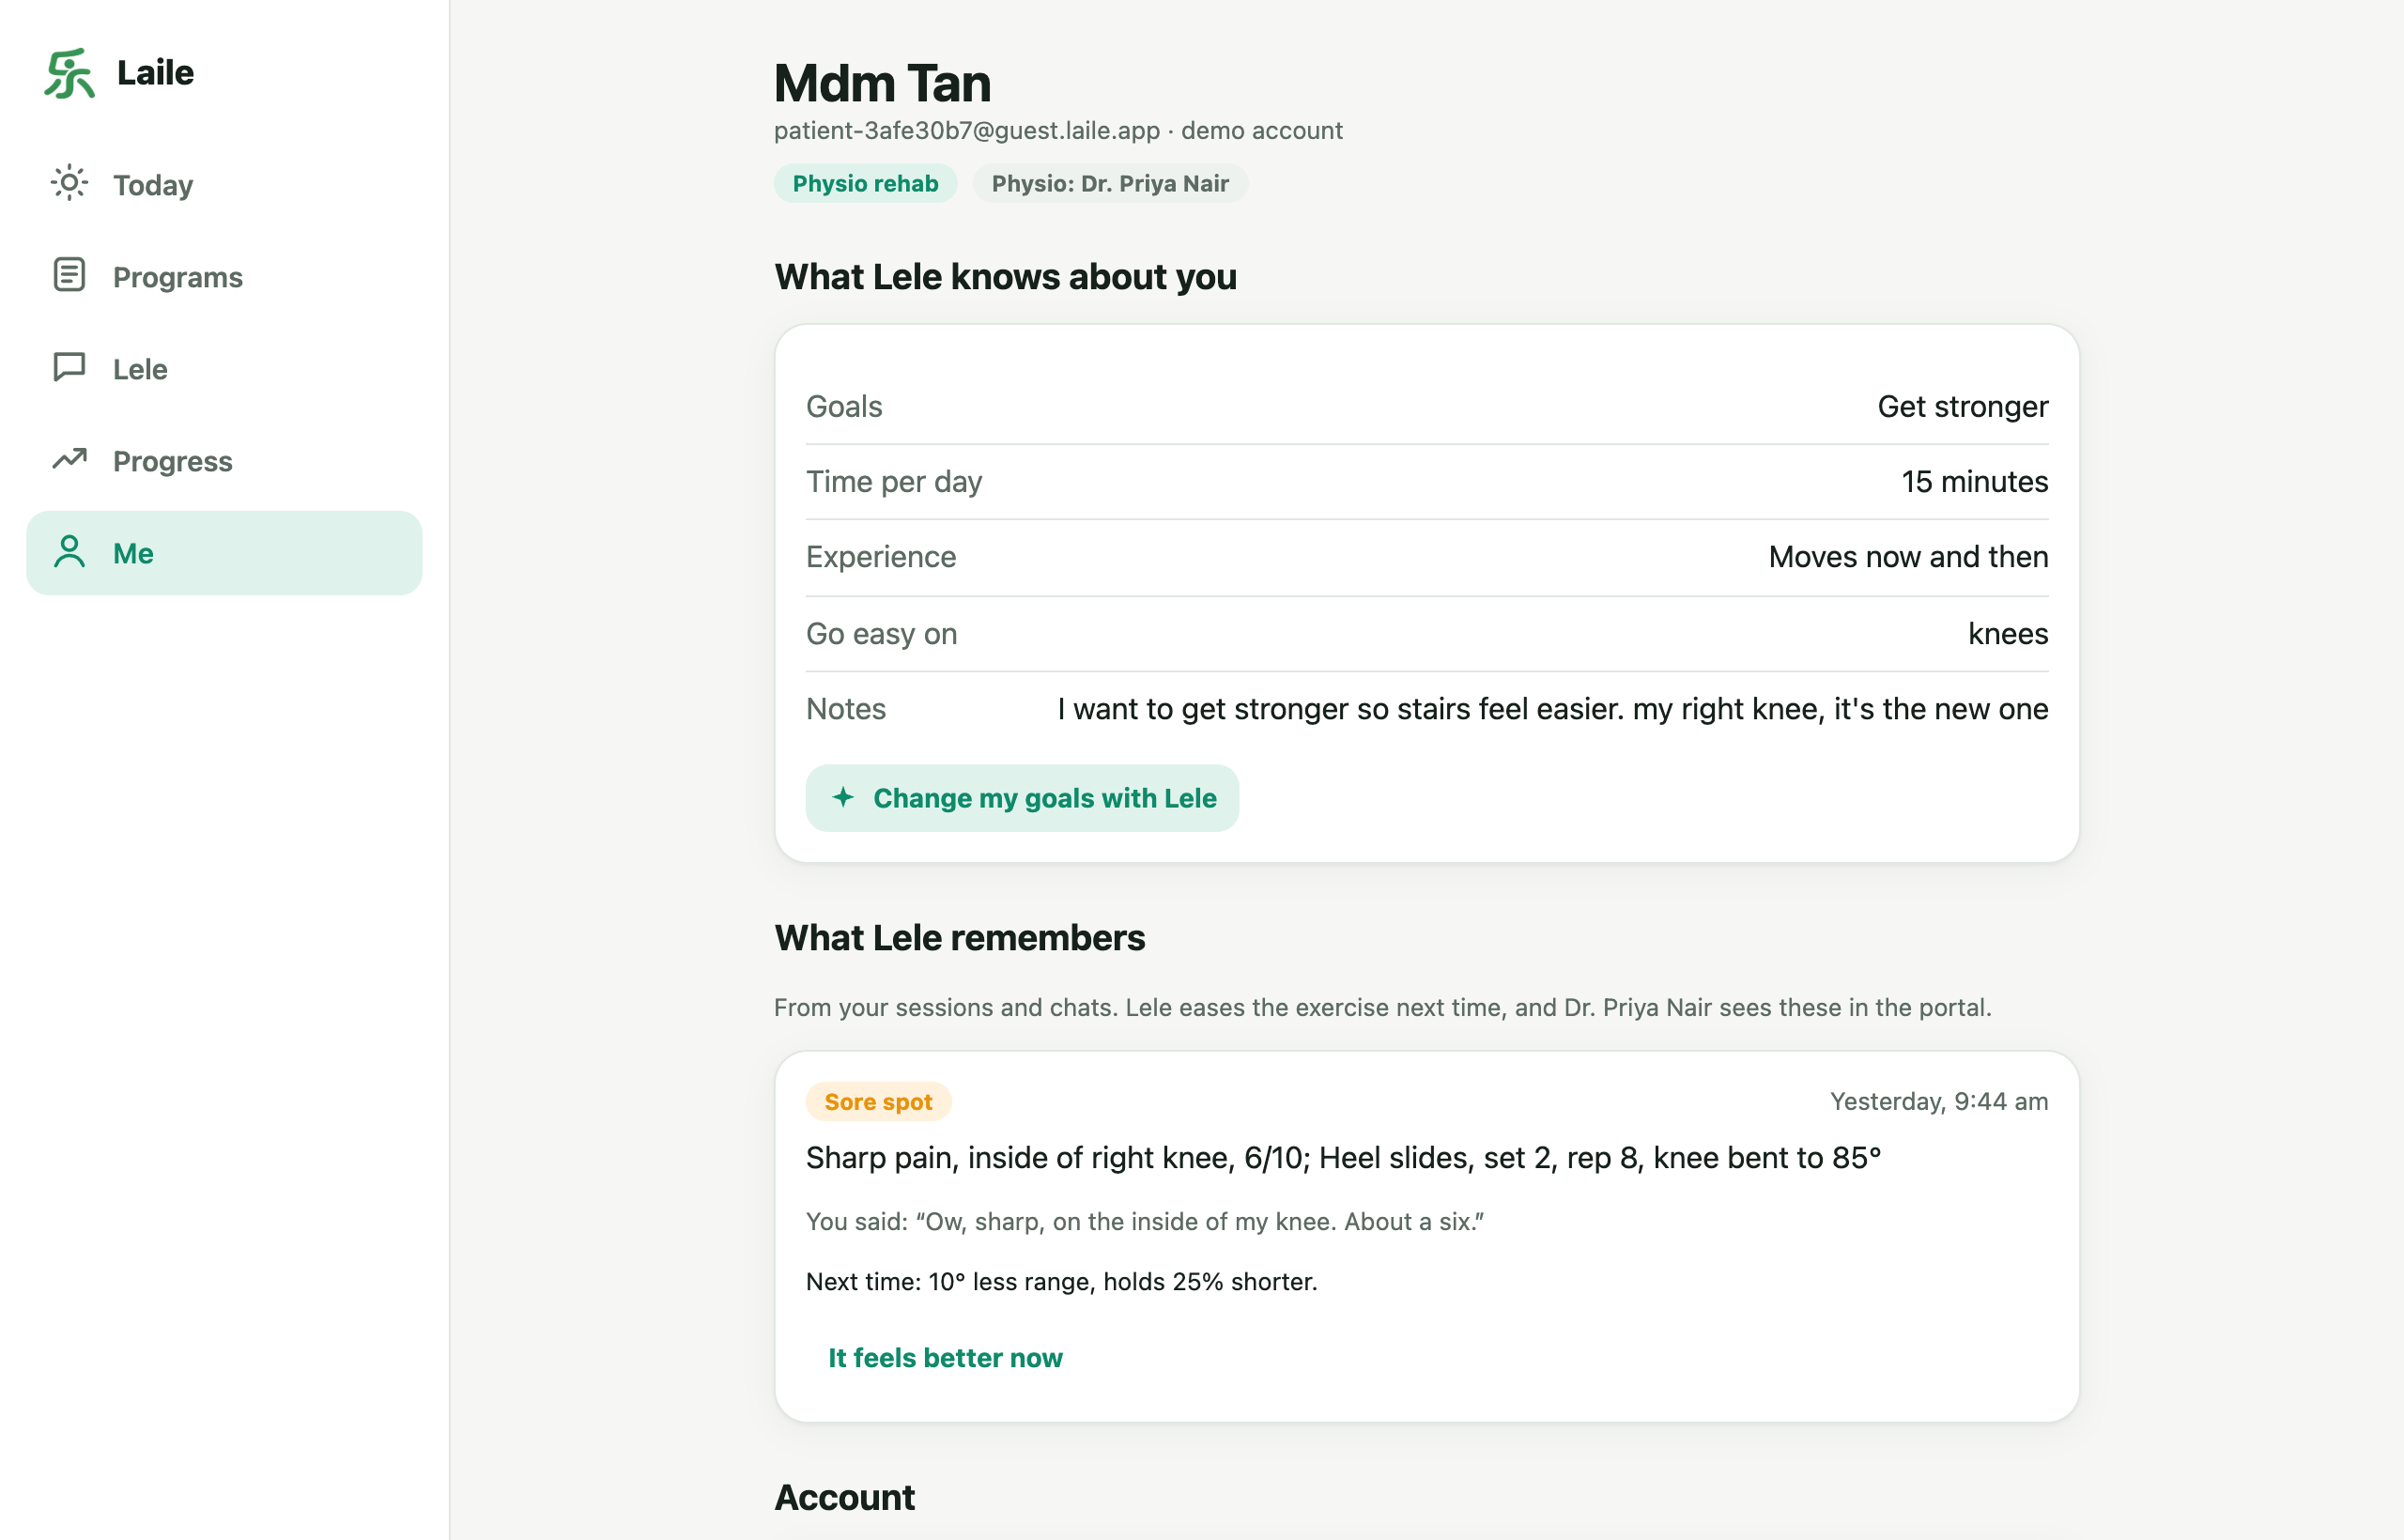
\includegraphics[width=0.49\linewidth]{../screenshots/32-web-me.png}}
\caption{Left: planning by chat; Lele drafted ``Gentle Strength for New Knee'' on ADP and sent it to Dr Nair to approve. Right: what Lele knows about the person and remembers from sessions.}
\end{figure}

\subsection{Medicines, explained and bounded}
Laile reminds people about doses their doctor scheduled and explains what each medicine is for and what to report, from a curated knowledge base. It never advises on starting, stopping, timing or dosing. Dose questions get a fixed referral to the doctor or pharmacist before any model sees them, and an unknown medicine gets ``I'm not able to identify that medication, please check with your pharmacist.''

\subsection{The physio stays on top}
The portal opens with \emph{Today from Lele}: red flags first, then people who felt worse this morning, pain reports to review, program requests (approve or say not yet), drafts to sign, missed days, barriers and upcoming visits. During a session the physio sees it live: exercise, reps and the measured angle every two seconds. Charts show each key measure against the person's baseline and milestones. The physio can ask Lele in plain words to change a program (``make it gentler, she had a flare''); Lele drafts a new version and nothing reaches the patient until the physio signs. Discharge hands the person to a follow-on program with any limits the physio chose to keep.

Each patient page opens with \emph{Lele's summary}: four to six lines that Lele on ADP writes from the person's record (adherence, the key measure with real numbers, what they reported, what is waiting for approval) and the knowledge base (what is typical at this stage after the procedure), ending with one thing worth discussing at the next visit. The numbers and flags are computed by Laile's code and passed in; the model only summarises them.

\begin{figure}[htbp]
\centering
\fbox{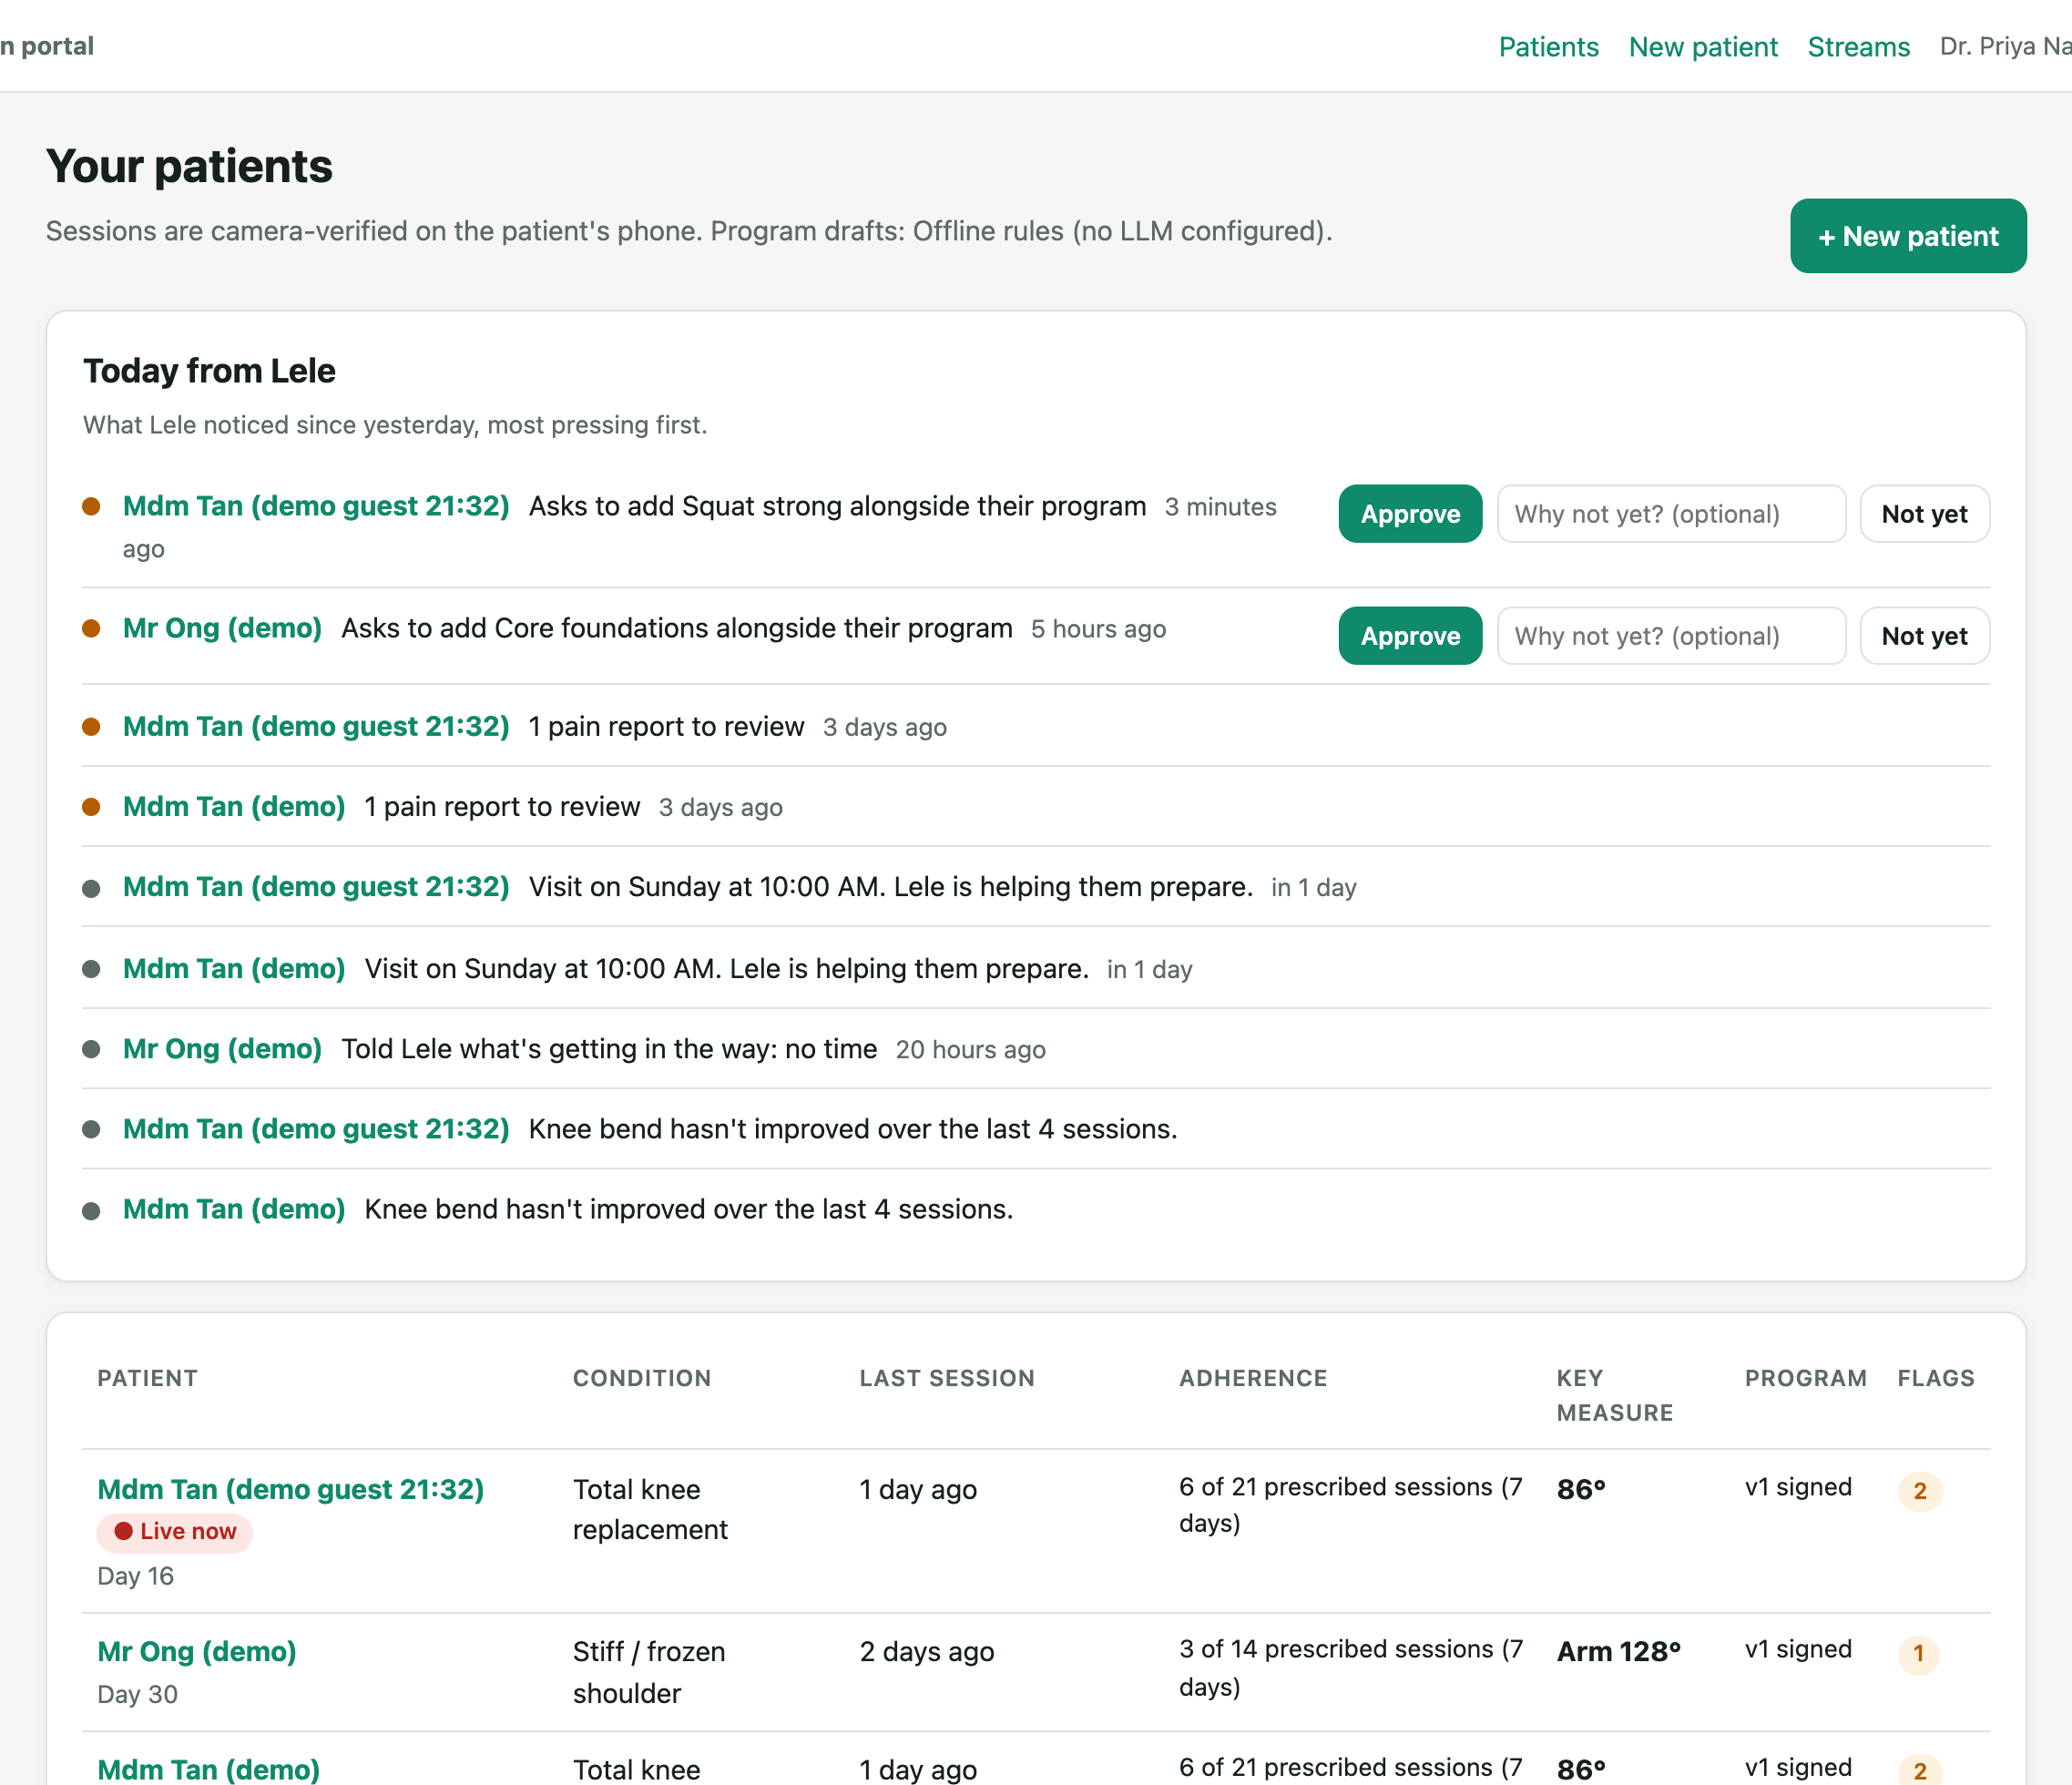
\includegraphics[width=0.97\linewidth,height=0.4\textheight,keepaspectratio]{../screenshots/20-portal-dashboard-crop.png}}
\caption{Today from Lele in the clinician portal: most pressing first, with approvals inline.}
\end{figure}
\begin{figure}[htbp]
\centering
\fbox{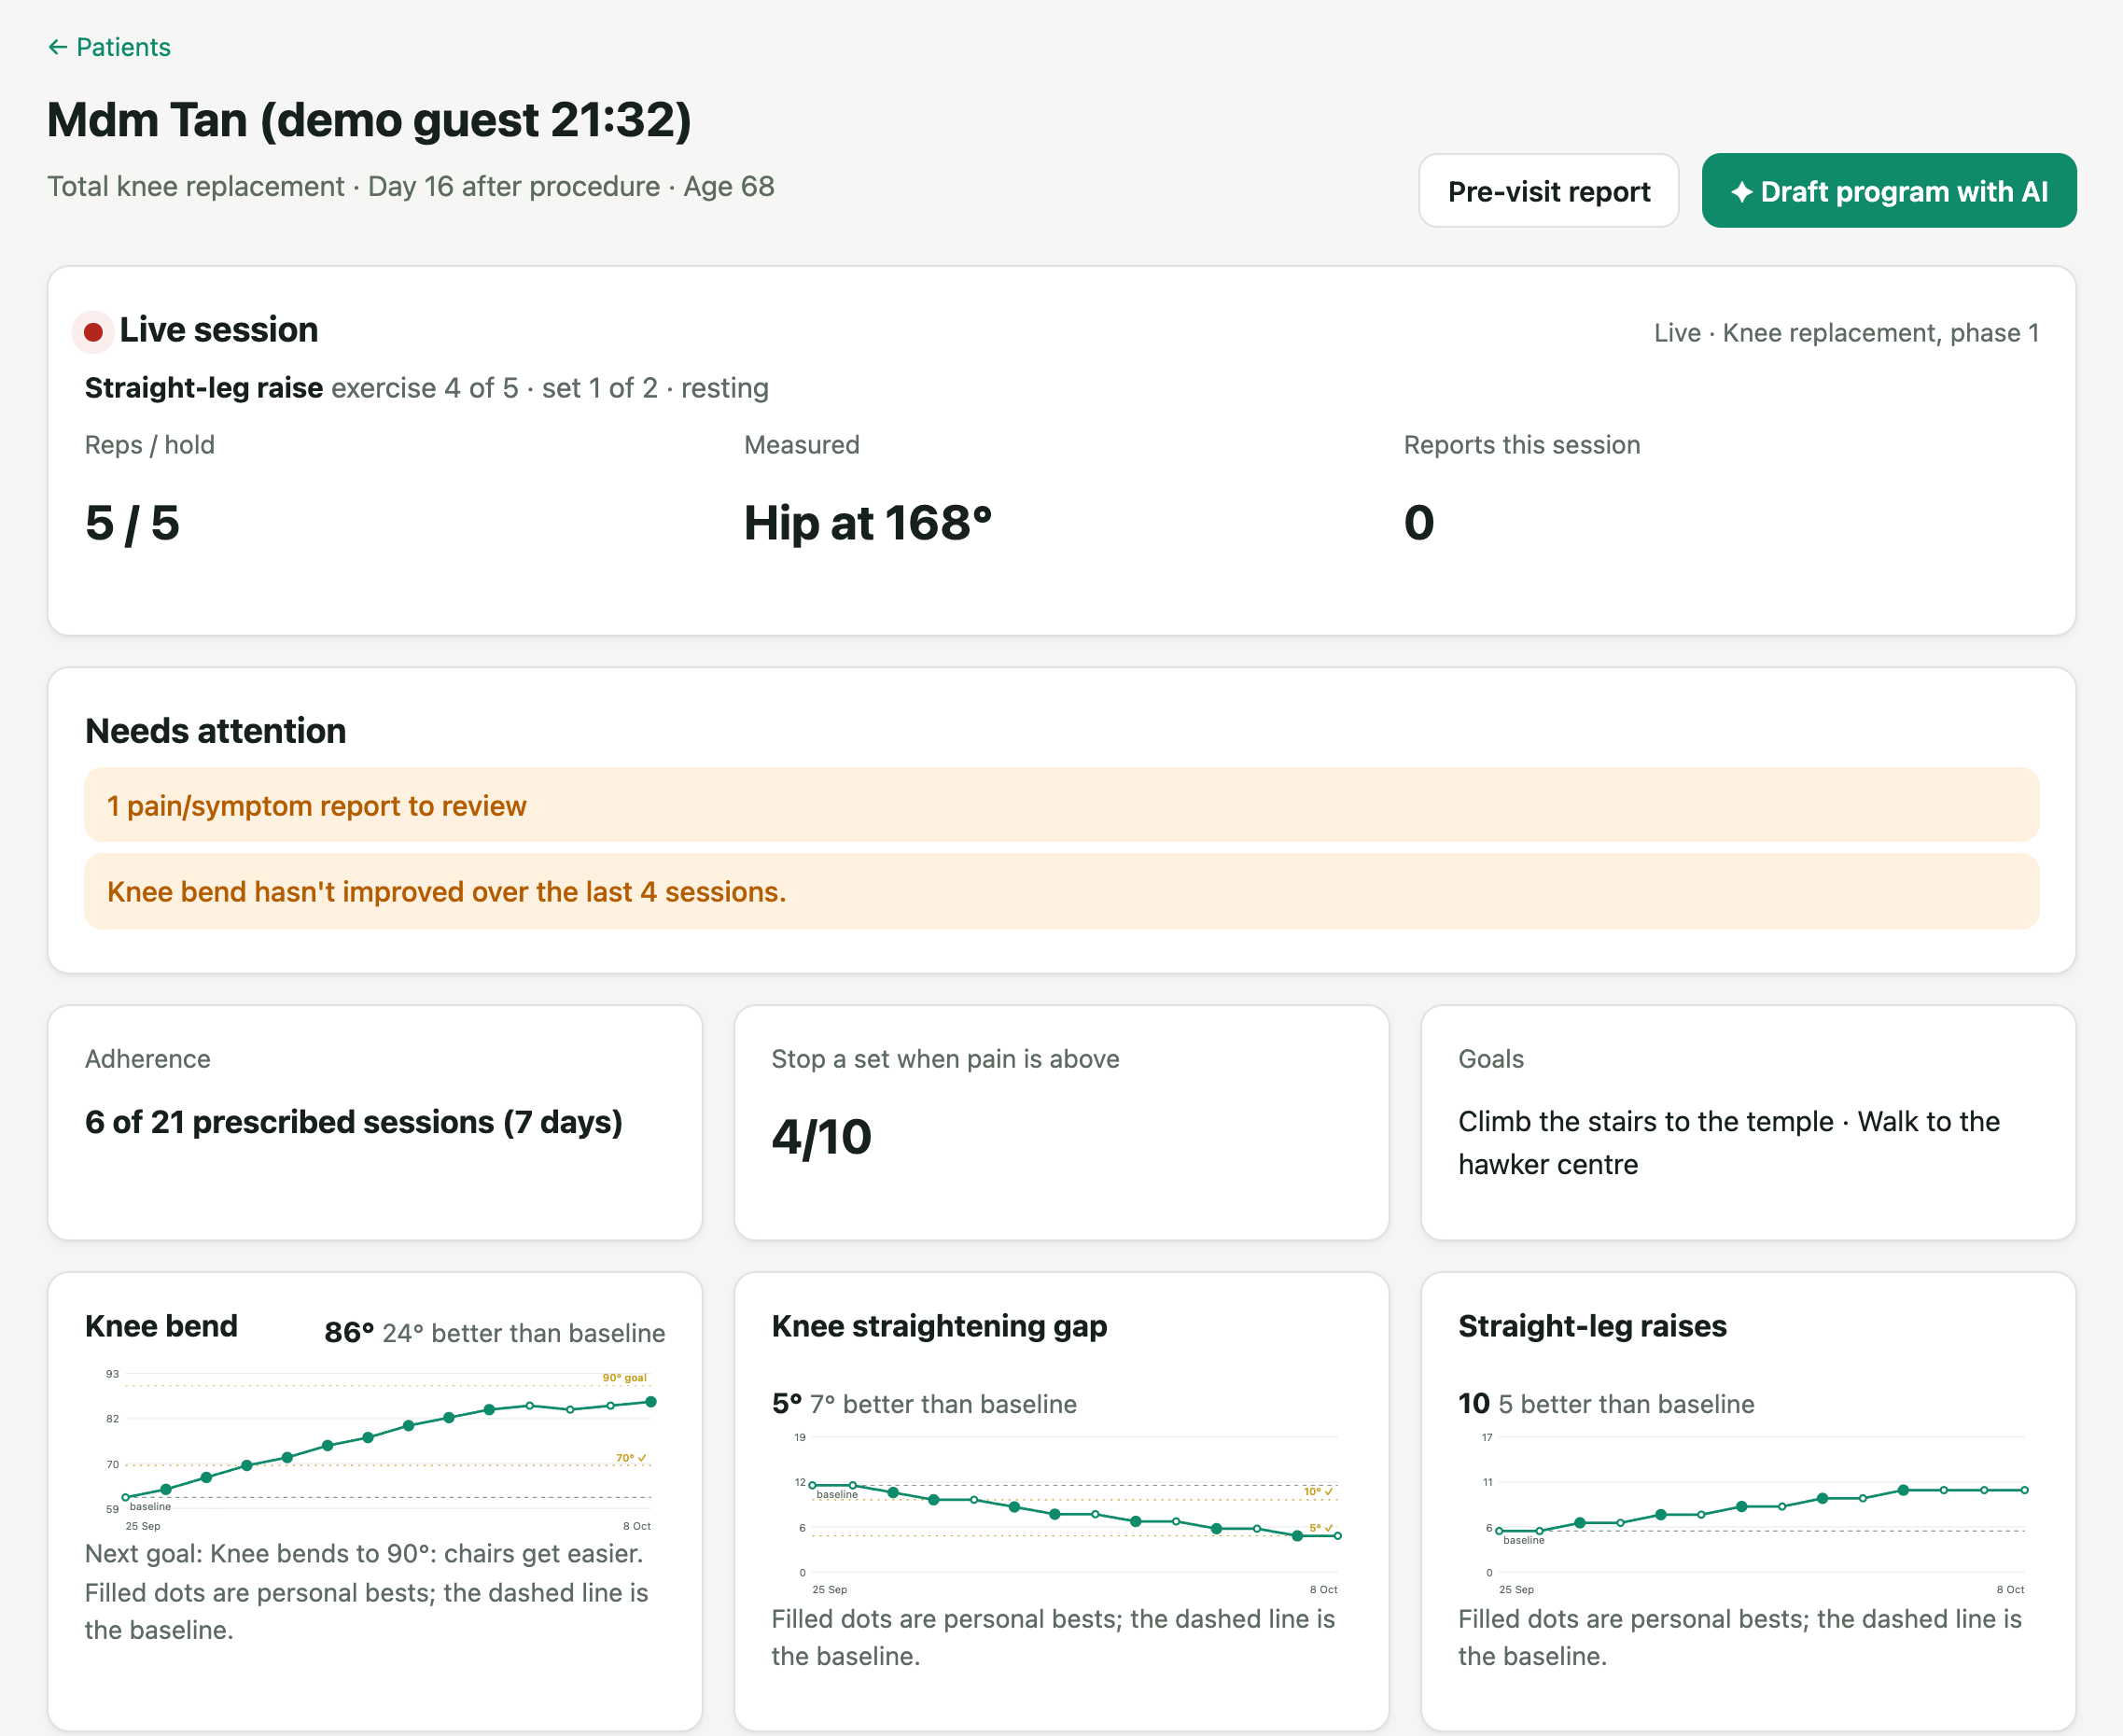
\includegraphics[width=0.97\linewidth,height=0.42\textheight,keepaspectratio]{../screenshots/21-portal-patient-crop.png}}
\caption{A patient's page: the session as it happens, what needs attention, and progress against baseline.}
\end{figure}
\begin{figure}[htbp]
\centering
\fbox{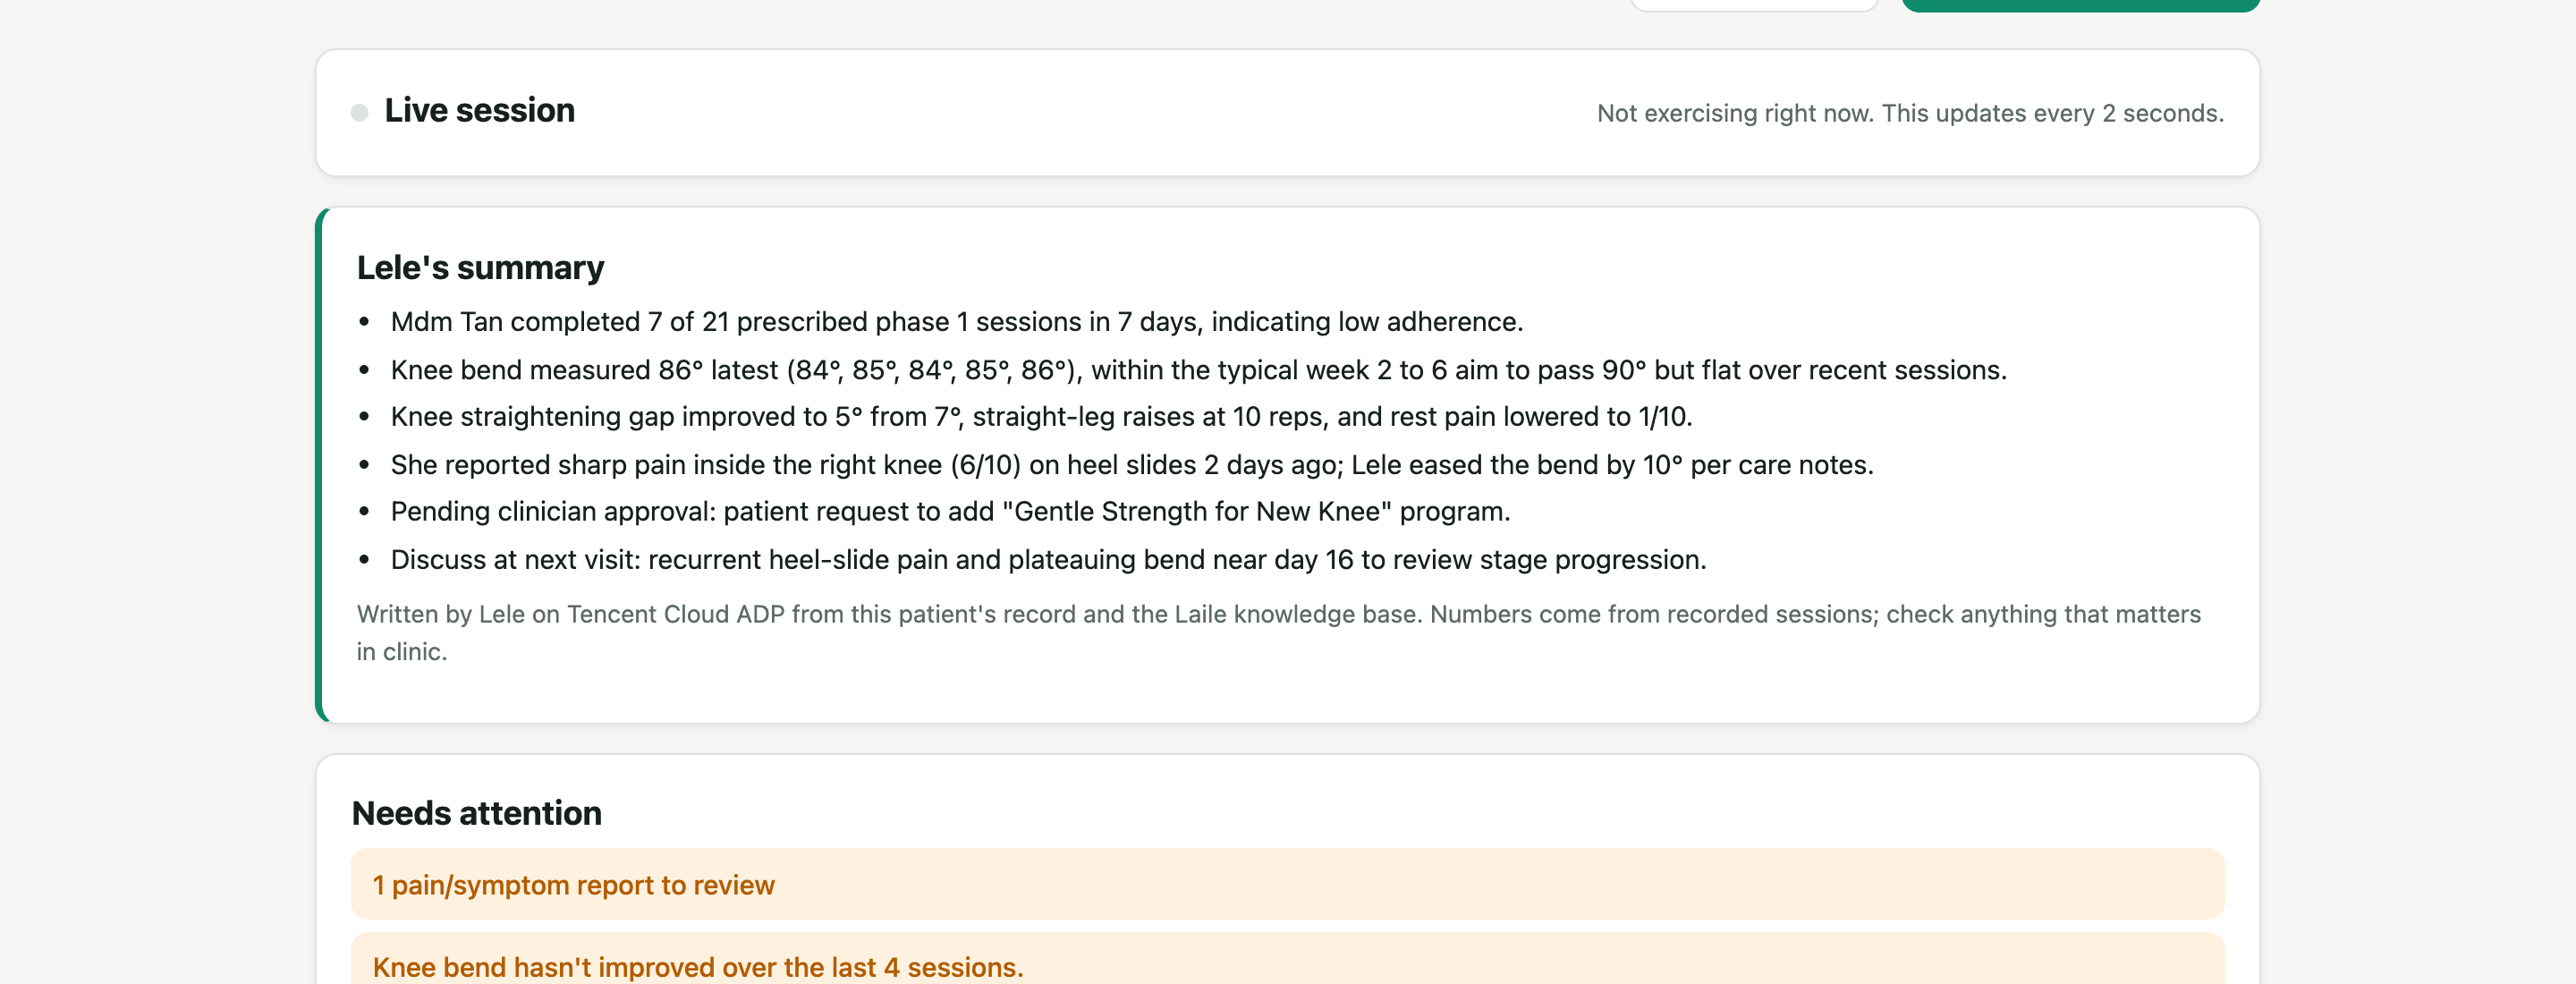
\includegraphics[width=0.97\linewidth]{../screenshots/35-portal-patient-brief-crop.png}}
\caption{Lele's summary for Dr Nair, written on Tencent Cloud ADP from Mdm Tan's record and the knowledge base (``typical week 2 to 6 aim to pass 90\textdegree'').}
\end{figure}

\subsection{Laile in the browser}
The same account works at \href{https://43-156-108-79.sslip.io/app}{43-156-108-79.sslip.io/app} on a laptop or any phone, with no install: Today, Programs, Lele (including planning by chat), Progress and Me. Sessions use the webcam with MediaPipe pose running in the browser, and a JavaScript port of Laile's session conductor, tested against the same plan the server sends, so a web session counts, pauses for pain, asks for a rating and reports to the physio exactly like a phone session. Lele speaks with the same ElevenLabs voice, and ``Tell Lele'' goes through the same safety rules.

\begin{center}
\begin{minipage}[t]{0.36\linewidth}\centering\fbox{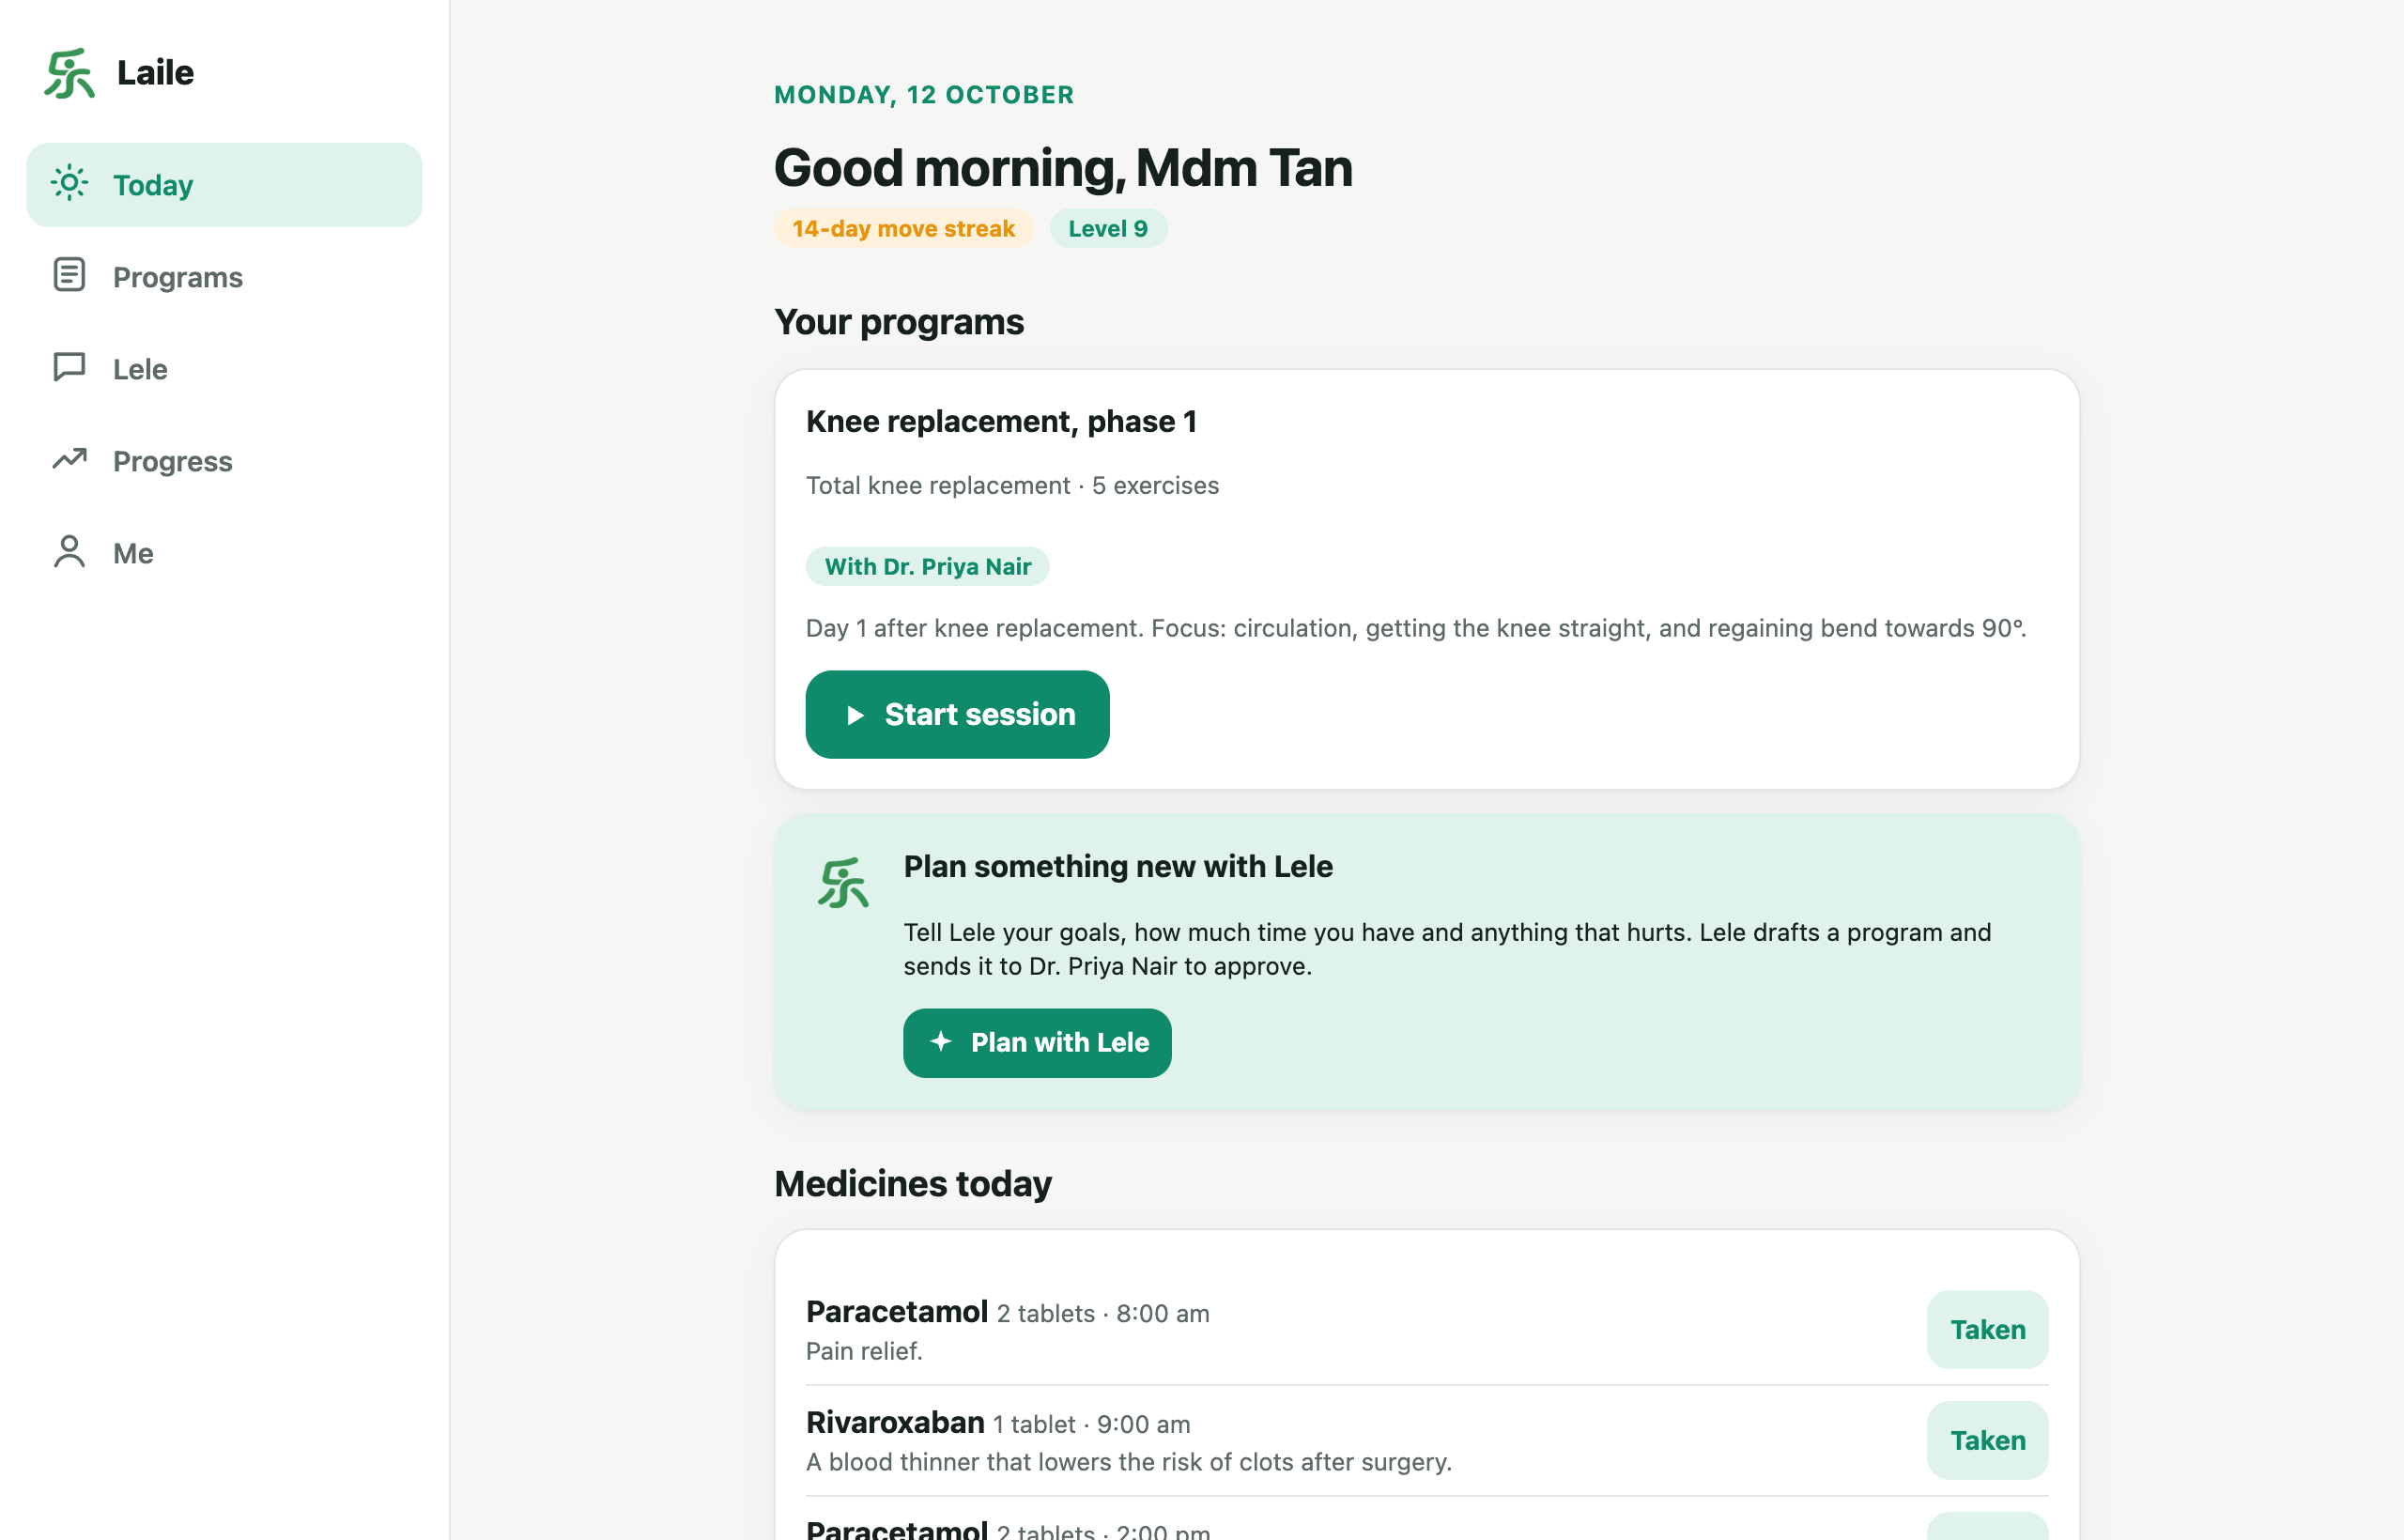
\includegraphics[width=\linewidth]{../screenshots/30-web-today.png}}\\[2pt]{\scriptsize\color{muted}Today on a laptop}\end{minipage}\hfill
\begin{minipage}[t]{0.36\linewidth}\centering\fbox{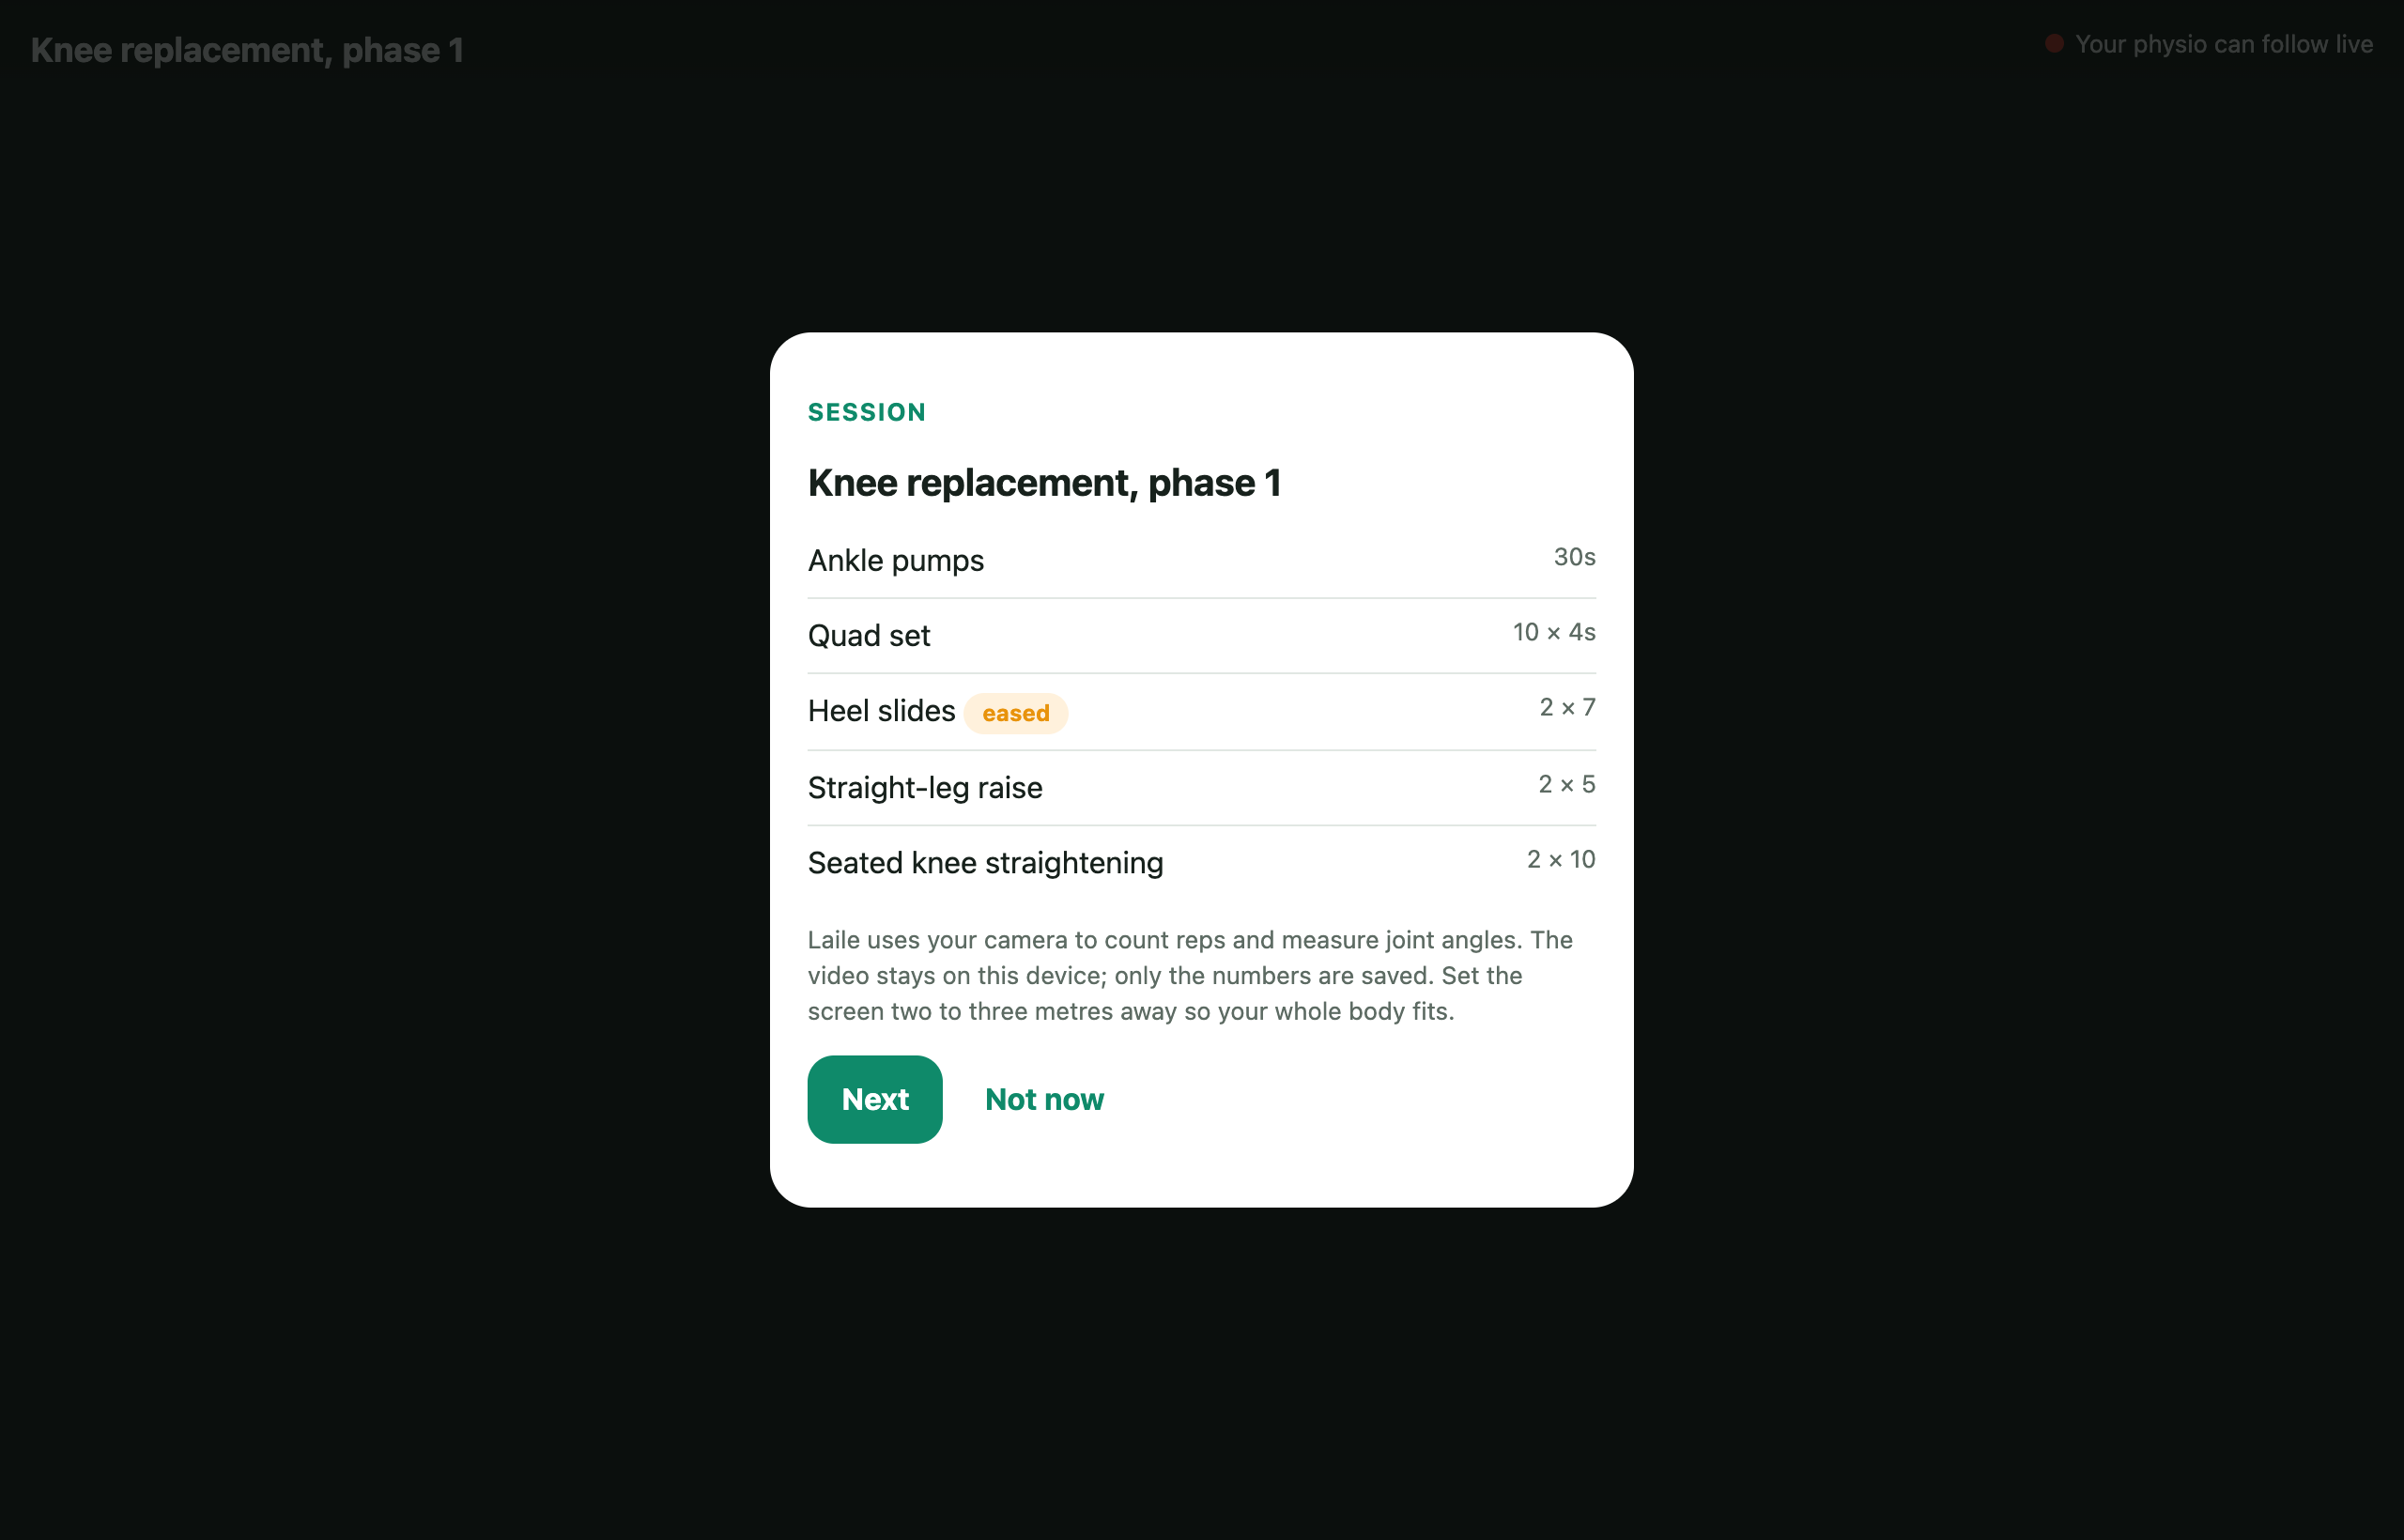
\includegraphics[width=\linewidth]{../screenshots/33-web-session.png}}\\[2pt]{\scriptsize\color{muted}A webcam session, heel slides eased by Lele}\end{minipage}\hfill
\begin{minipage}[t]{0.16\linewidth}\centering\fbox{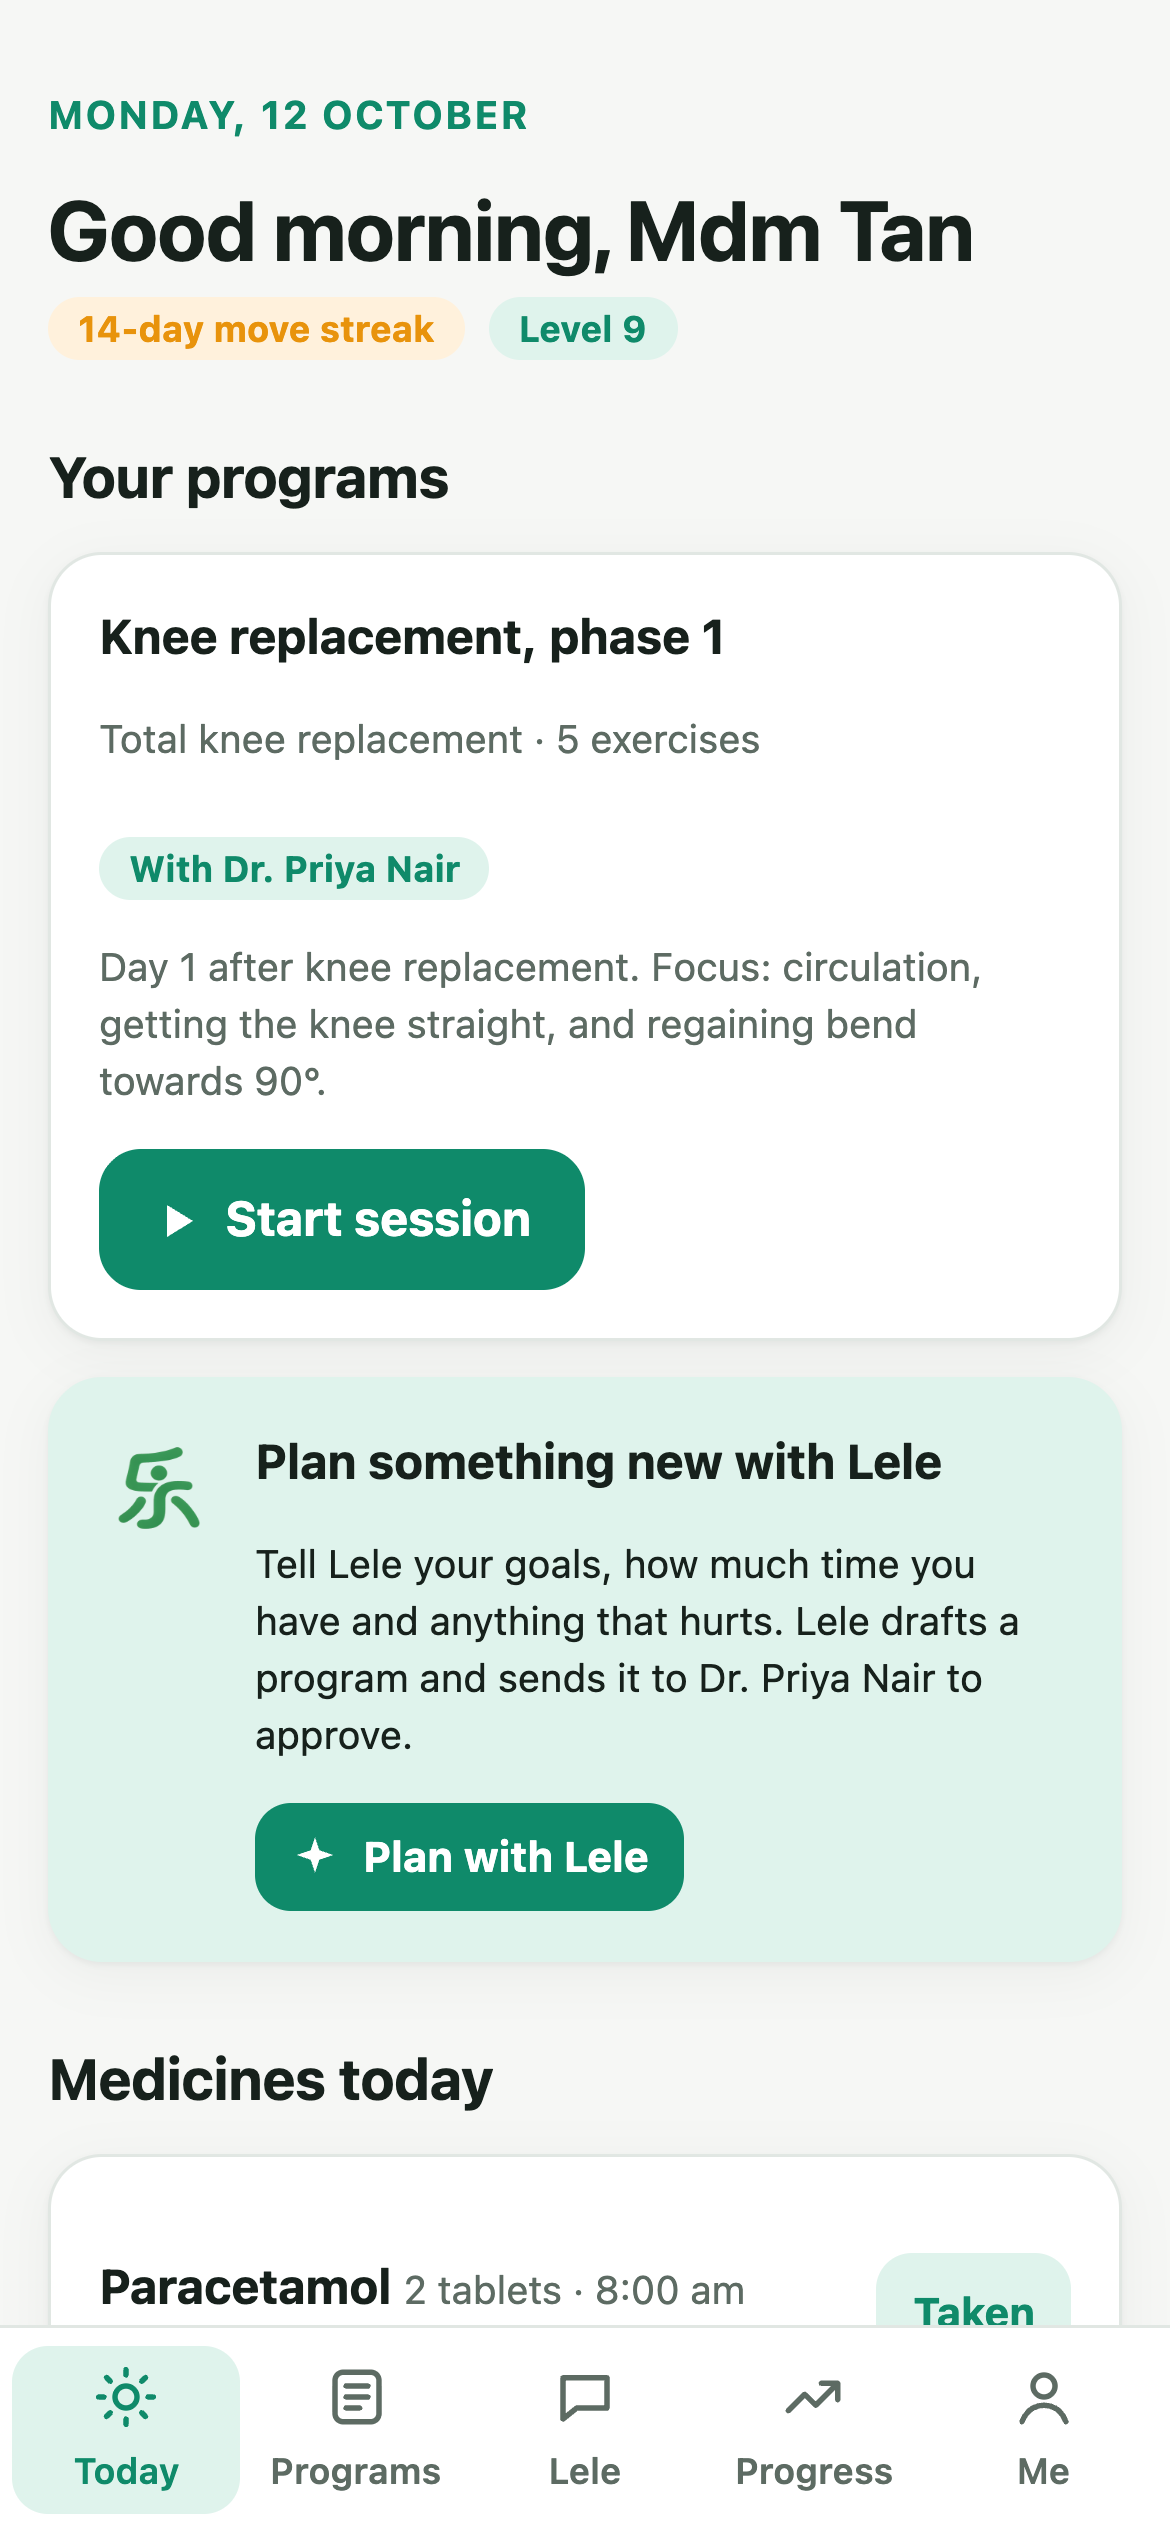
\includegraphics[width=\linewidth]{../screenshots/34-web-today-phone.png}}\\[2pt]{\scriptsize\color{muted}On a phone}\end{minipage}
\end{center}

\section{How the AI is used}
\begin{tabularx}{\linewidth}{@{}L{3.6cm}L{4.6cm}Y@{}}
\toprule
\textbf{Job} & \textbf{Done by} & \textbf{Kept safe by}\\
\midrule
Conversation, explanations, progress reviews & Lele agent on \textbf{Tencent Cloud ADP} (Hy3 model, knowledge base of 12 documents in two categories, persona prompt) & Server sends real context (program, measurements, care notes); red flags and dose questions answered by fixed rules first; fallback reply when the knowledge base has no answer\\
Remembering what hurt & Lele (care notes; model can propose a note as structured JSON) & Notes are validated and stored by code; easing is computed by \texttt{CareMemory}, never by the model\\
Program drafts (portal, Lele's plans, revisions) & Lele on \textbf{Tencent Cloud ADP} (\texttt{PLAN REQUEST} mode, using the knowledge base); rule-based drafter as fallback & Only exercises in the vetted library, dose limits enforced, contraindication checker removes anything a precaution rules out; physio signs or approves\\
Brief for the physio & Lele on \textbf{Tencent Cloud ADP} (\texttt{CLINICIAN BRIEF} mode) with the patient's record and the knowledge base & Every number and flag is computed by code and passed in; labelled as Lele's summary to check in clinic\\
Understanding replies & \texttt{ReplyReader} and \texttt{GoalsReader} (keyword rules) & Shows ``Lele heard: \ldots''; asks again when unclear\\
Seeing movement & Apple Vision on iPhone; MediaPipe pose in the browser & Video stays on the device; no count when the camera can't see the joint\\
Lele's voice & ElevenLabs on phone and web, cached per line on the server & Phone falls back to its own voice; counts never wait on the network\\
\bottomrule
\end{tabularx}

\section{Architecture and trust boundary}
\begin{center}
\resizebox{\linewidth}{!}{% Laile architecture and trust boundary. Included by architecture.tex, the write-up and the deck.
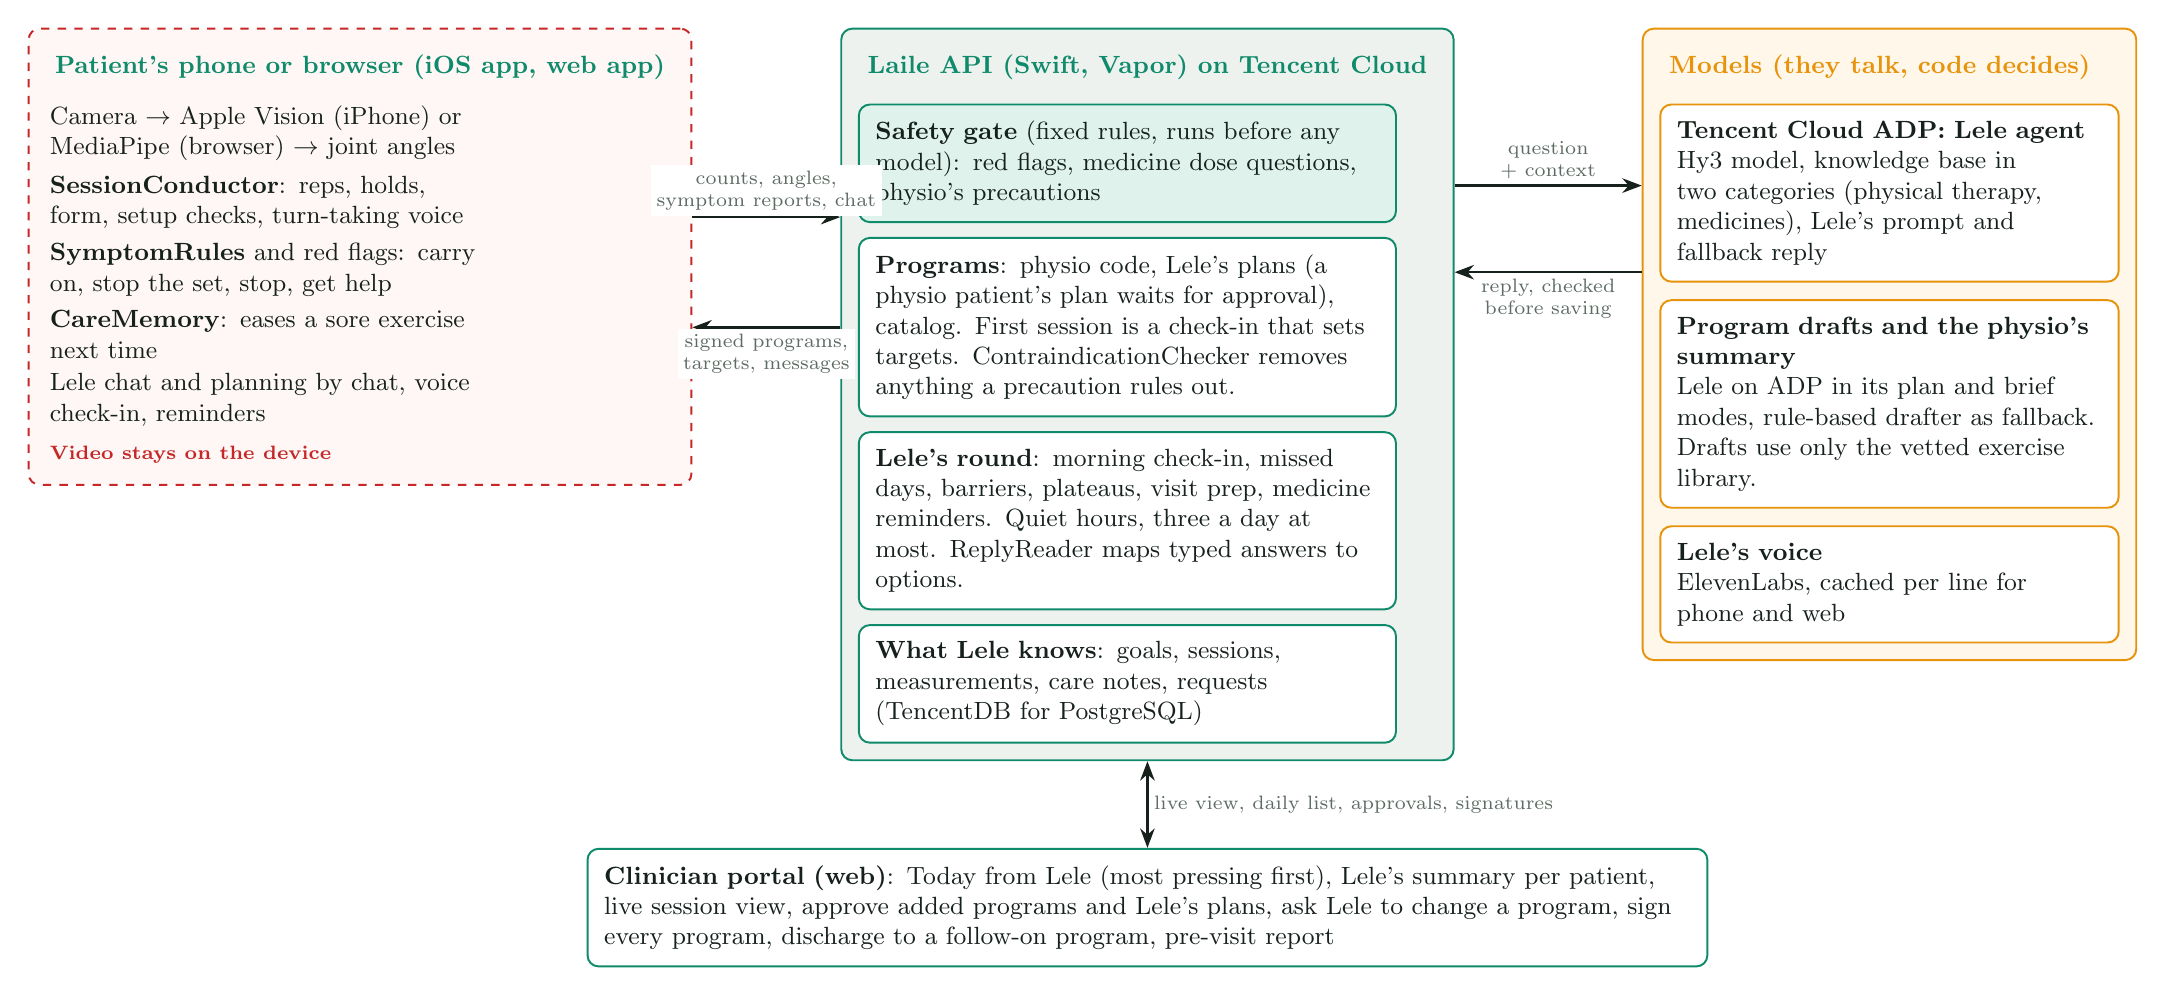
\begin{tikzpicture}[
    font=\small,
    every node/.style={text=ink, execute at begin node={\hyphenpenalty=10000\exhyphenpenalty=10000}},
    box/.style={draw=#1, fill=white, rounded corners=4pt, line width=0.7pt, align=left, inner sep=6pt},
    box/.default=accent,
    item/.style={align=left, text width=#1, inner sep=1.5pt},
    item/.default=5.6cm,
    title/.style={font=\small\bfseries, align=left},
    flow/.style={-{Stealth[length=7pt]}, line width=0.9pt, draw=ink},
    lab/.style={font=\scriptsize, text=muted, fill=white, inner sep=2pt, align=center},
  ]

  % --- Phone -------------------------------------------------------------
  \node[title, text=accent] (phoneT) at (0,0) {Patient's phone or browser (iOS app, web app)};
  \node[item, below=4pt of phoneT.south west, anchor=north west] (p1) {Camera $\rightarrow$ Apple Vision (iPhone) or MediaPipe (browser) $\rightarrow$ joint angles};
  \node[item, below=2pt of p1.south west, anchor=north west] (p2) {\textbf{SessionConductor}: reps, holds, form, setup checks, turn-taking voice};
  \node[item, below=2pt of p2.south west, anchor=north west] (p3) {\textbf{SymptomRules} and red flags: carry on, stop the set, stop, get help};
  \node[item, below=2pt of p3.south west, anchor=north west] (p4) {\textbf{CareMemory}: eases a sore exercise next time};
  \node[item, below=2pt of p4.south west, anchor=north west] (p5) {Lele chat and planning by chat, voice check-in, reminders};
  \node[item, below=4pt of p5.south west, anchor=north west, text=danger, font=\scriptsize\bfseries] (p6) {Video stays on the device};
  \begin{scope}[on background layer]
    \node[box=danger, dashed, fit=(phoneT)(p1)(p2)(p3)(p4)(p5)(p6), fill=dangersoft!35] (phone) {};
  \end{scope}

  % --- Laile API -----------------------------------------------------------
  \node[title, text=accent] (apiT) at (10.0,0) {Laile API (Swift, Vapor) on Tencent Cloud};
  \node[box, fill=accentsoft, below=5pt of apiT.south west, anchor=north west, text width=6.4cm] (gate)
    {\textbf{Safety gate} (fixed rules, runs before any model): red flags, medicine dose questions, physio's precautions};
  \node[box, below=5pt of gate, text width=6.4cm] (prog)
    {\textbf{Programs}: physio code, Lele's plans (a physio patient's plan waits for approval), catalog. First session is a check-in that sets targets. ContraindicationChecker removes anything a precaution rules out.};
  \node[box, below=5pt of prog, text width=6.4cm] (round)
    {\textbf{Lele's round}: morning check-in, missed days, barriers, plateaus, visit prep, medicine reminders. Quiet hours, three a day at most. ReplyReader maps typed answers to options.};
  \node[box, below=5pt of round, text width=6.4cm] (data)
    {\textbf{What Lele knows}: goals, sessions, measurements, care notes, requests (TencentDB for PostgreSQL)};
  \begin{scope}[on background layer]
    \node[box, fit=(apiT)(gate)(prog)(round)(data), fill=surface] (api) {};
  \end{scope}

  % --- AI services ---------------------------------------------------------
  \node[title, text=reward] (aiT) at (19.3,0) {Models (they talk, code decides)};
  \node[box=reward, below=5pt of aiT.south west, anchor=north west, text width=5.4cm] (adp)
    {\textbf{Tencent Cloud ADP: Lele agent}\\ Hy3 model, knowledge base in two categories (physical therapy, medicines), Lele's prompt and fallback reply};
  \node[box=reward, below=6pt of adp, text width=5.4cm] (hy)
    {\textbf{Program drafts and the physio's summary}\\ Lele on ADP in its plan and brief modes, rule-based drafter as fallback. Drafts use only the vetted exercise library.};
  \node[box=reward, below=6pt of hy, text width=5.4cm] (voice)
    {\textbf{Lele's voice}\\ ElevenLabs, cached per line for phone and web};
  \begin{scope}[on background layer]
    \node[box=reward, fit=(aiT)(adp)(hy)(voice), fill=rewardsoft!60] (ai) {};
  \end{scope}

  % --- Portal --------------------------------------------------------------
  \node[box, below=1.1cm of api, text width=13.8cm, xshift=0cm] (portal)
    {\textbf{Clinician portal (web)}: Today from Lele (most pressing first), Lele's summary per patient, live session view, approve added programs and Lele's plans, ask Lele to change a program, sign every program, discharge to a follow-on program, pre-visit report};

  % --- Flows (horizontal, at fixed heights) ------------------------------------
  \draw[flow] (phone.east |- 0,-1.9) -- node[lab, above, pos=0.5] {counts, angles,\\symptom reports, chat} (api.west |- 0,-1.9);
  \draw[flow] (api.west |- 0,-3.3) -- node[lab, below, pos=0.5] {signed programs,\\targets, messages} (phone.east |- 0,-3.3);
  \draw[flow] (api.east |- 0,-1.5) -- node[lab, above, pos=0.5] {question\\+ context} (ai.west |- 0,-1.5);
  \draw[flow] (ai.west |- 0,-2.6) -- node[lab, below, pos=0.5] {reply, checked\\before saving} (api.east |- 0,-2.6);
  \draw[flow, {Stealth[length=7pt]}-{Stealth[length=7pt]}] (api.south) -- node[lab, right] {live view, daily list, approvals, signatures} (portal.north -| api.south);
\end{tikzpicture}
}
\end{center}

\textbf{Design rules.}
\begin{enumerate}[leftmargin=1.4em]
  \item \textbf{The model talks; code decides.} Counting, timing, pain thresholds, escalation, easing and every number a clinician sees come from deterministic, tested code.
  \item \textbf{The AI never prescribes.} Only physio-signed programs reach a supervised patient. Drafts use the vetted library within dose limits, and anything that breaks a precaution is removed before a person sees it.
  \item \textbf{Honest about uncertainty.} No camera view, no count (``I can't see you clearly, so I'm not counting that''). An ambiguous remark gets ``stretch or sharp pain?''. An unclear typed answer gets asked again.
  \item \textbf{Memory is a record.} Care notes live in Laile's database with a history line for every change, visible to the person and the physio.
  \item \textbf{One codebase.} The phone and the server run the same Swift domain package (\texttt{LaileCore}), so safety rules work offline and the server re-checks with the same engine.
\end{enumerate}

\textbf{Key trade-offs.}

\begin{tabularx}{\linewidth}{@{}L{4.2cm}Y@{}}
\toprule
\textbf{Choice} & \textbf{Why, and what it costs}\\
\midrule
Native iOS (SwiftUI), a web app and a Swift server & Native camera and Vision performance and one language for the domain logic. The web app covers Android phones and laptops with no install; its session engine is a JavaScript port of the Swift one, kept honest by tests against the same plan.\\
Pose on the device (Vision, MediaPipe) & No video upload; the iPhone needs no model download and works offline. Joints are 2D, so angles are camera estimates for tracking trends (stated on every report).\\
Fixed rules for safety, model for conversation & Predictable, testable safety. Unusual phrasings fall back to a clarifying question.\\
ADP knowledge base for explanations & Curated, reviewable content and Tencent's guardrails. ADP's answer template can be verbose, so the server trims headings and citations.\\
Server-rendered portal & Fast to build, prints cleanly as a pre-visit report, no second front-end stack.\\
\bottomrule
\end{tabularx}

\section{Fit with the challenge}\label{sec:fit}
\begin{tabularx}{\linewidth}{@{}L{3.6cm}Y@{}}
\toprule
\textbf{The brief asks for} & \textbf{In Laile}\\
\midrule
Medication understanding & ``What's this for?'' on every dose; Lele explains from the medicines knowledge base\\
Medication management & Reminders at the doctor's times (in the app and as notifications); one tap or a typed reply marks a dose taken\\
Adherence support & Camera-verified sessions, check-in targets, streaks that forgive one missed day, Lele's barrier questions and nudges\\
Health tracking & Knee bend, straightening gap, arm lift, reps, holds and pain over time, against baseline and milestones\\
Preventive health & Precautions follow the person everywhere; plateau and missed-day flags; follow-on programs after discharge; red-flag rules\\
Healthcare preparation & Visit prep questions from sessions and notes; pre-visit report and Lele's summary for the physio\\
Empowering, personalised, longitudinal & Goals in their own words, new plans by chatting with Lele, targets from their own check-in, a record of each person that builds over weeks\\
Safe, strictly bounded, honest & Fixed referral for dose questions, red flags handled by rules, ``I'm not able to identify that medication, please check with your pharmacist''\\
\bottomrule
\end{tabularx}

\section{Responsible AI}
\begin{itemize}
  \item \textbf{Privacy.} Video stays on the phone or in the browser; Laile stores joint angles, counts and what the person reports. Linking to a physio needs the patient's code and consent, and shares data with that physio only.
  \item \textbf{Clinical safety.} Red-flag phrases (chest pain, a swollen hot calf, fainting and others) end the session with clear advice to call 995 or contact the care team, whatever any model says. Pain above the physio's limit stops the set.
  \item \textbf{Human in the loop.} Physios sign programs, approve additions and Lele's plans, and decide discharge. Lele's daily list and summary help them prioritise and change nothing on their own.
  \item \textbf{No nagging.} Quiet hours, a daily limit on conversations Lele starts, and no repeated messages.
  \item \textbf{Known limits.} The knowledge base is general education and needs review by a physiotherapist and a pharmacist before real patients use it. Camera angles are estimates. Laile has not been clinically validated.
\end{itemize}

\section{Business value}
\begin{itemize}
  \item \textbf{Clinics pay for visibility.} Physiotherapy clinics and hospital rehabilitation teams get verified adherence, live sessions and a prioritised daily list without extra visits. Proposed model: a monthly fee per active patient (to be validated with clinics).
  \item \textbf{People stay after discharge.} Discharge hands patients to a calisthenics or mobility program with their limits carried over. That keeps the habit going and turns a clinical episode into a long-term relationship, with a consumer subscription for people without a physio.
  \item \textbf{Each side feeds the other.} Everyday users with aches are pointed to a physio; physio patients become everyday users afterwards.
  \item \textbf{Low running cost.} Pose estimation runs on the phone, model calls are only for conversation, and voice lines are cached and paid for once.
  \item \textbf{Fit for Singapore.} An ageing population and a national push towards preventive care favour tools that keep older adults strong at home.
\end{itemize}

\section{Status and next steps}
\textbf{Working today.} The iOS app (Today, Programs, Lele, Progress) on TestFlight with a public link; the web app with webcam sessions; the server and clinician portal on Tencent Cloud Lighthouse; Lele published on Tencent Cloud ADP, answering chat, drafting programs and writing the physio's summary; planning by chat with physio approval; demo accounts with realistic history; and 158 automated tests (121 for the shared domain package, 32 for the server, 5 for the web session engine).

\textbf{Next.} Move records to TencentDB for PostgreSQL; test with people at home (camera placement, lighting, rep thresholds, voice across a room); have a physiotherapist and a pharmacist review the knowledge base; pilot with one clinic.

\section{How it was built}
\laile\ is a Swift monorepo: \texttt{LaileCore} (pure Swift domain logic shared by phone and server), \texttt{LaileKit} (SwiftUI feature modules), the iOS app, a Vapor server with the clinician portal, and the web app (plain JavaScript modules served by the same server, no build step). Lele's prompt and knowledge base live in \texttt{agent/} and are imported into ADP.

\begin{figure}[htbp]
\centering
\resizebox{\linewidth}{!}{% Laile's tech stack in three columns. Included by the write-up and the deck.
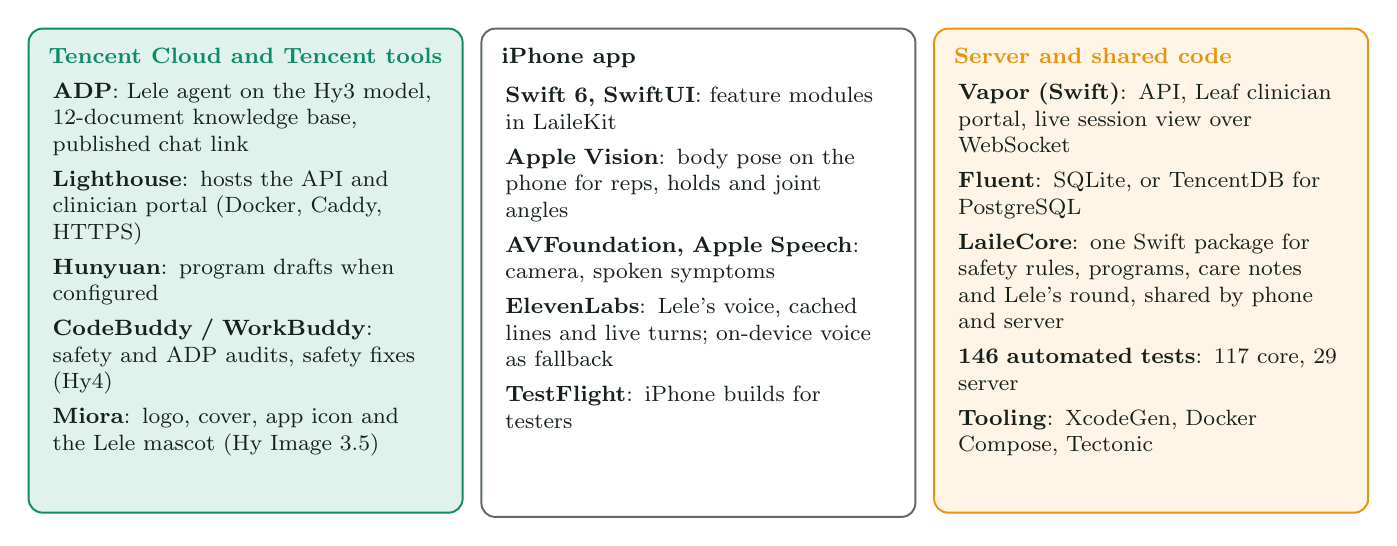
\begin{tikzpicture}[
    font=\fontsize{8}{9.6}\selectfont,
    every node/.style={text=ink, execute at begin node={\hyphenpenalty=10000\exhyphenpenalty=10000}},
    head/.style={font=\fontsize{8.5}{10}\selectfont\bfseries, text=#1, align=left, anchor=north west, inner sep=0pt},
    item/.style={align=left, anchor=north west, text width=4.9cm, inner sep=1.5pt},
    group/.style={draw=#1, rounded corners=5pt, line width=0.7pt, inner sep=7pt},
  ]
  \newcommand{\stackcol}[5]{%
    % #1 x, #2 name, #3 colour, #4 title, #5 items
    \node[head=#3] (#2-t) at (#1,0) {#4};
    \node[item, below=5pt of #2-t.south west, anchor=north west] (#2-b) {\parbox[t][5.15cm][t]{4.9cm}{#5}};
  }

  \stackcol{0}{tc}{accent}{Tencent Cloud and Tencent tools}{%
    \textbf{ADP}: Lele agent on the Hy3 model, 12-document knowledge base, published chat link\\[3pt]
    \textbf{Lighthouse}: hosts the API and clinician portal (Docker, Caddy, HTTPS)\\[3pt]
    \textbf{Hunyuan}: program drafts when configured\\[3pt]
    \textbf{CodeBuddy / WorkBuddy}: safety and ADP audits, safety fixes (Hy4)\\[3pt]
    \textbf{Miora}: logo, cover, app icon and the Lele mascot (Hy Image 3.5)}

  \stackcol{5.75}{ph}{ink}{iPhone app}{%
    \textbf{Swift 6, SwiftUI}: feature modules in LaileKit\\[3pt]
    \textbf{Apple Vision}: body pose on the phone for reps, holds and joint angles\\[3pt]
    \textbf{AVFoundation, Apple Speech}: camera, spoken symptoms\\[3pt]
    \textbf{ElevenLabs}: Lele's voice, cached lines and live turns; on-device voice as fallback\\[3pt]
    \textbf{TestFlight}: iPhone builds for testers}

  \stackcol{11.5}{sv}{reward}{Server and shared code}{%
    \textbf{Vapor (Swift)}: API, Leaf clinician portal, live session view over WebSocket\\[3pt]
    \textbf{Fluent}: SQLite, or TencentDB for PostgreSQL\\[3pt]
    \textbf{LaileCore}: one Swift package for safety rules, programs, care notes and Lele's round, shared by phone and server\\[3pt]
    \textbf{146 automated tests}: 117 core, 29 server\\[3pt]
    \textbf{Tooling}: XcodeGen, Docker Compose, Tectonic}

  \begin{scope}[on background layer]
    \node[group=accent, fill=accentsoft, fit=(tc-t)(tc-b)] {};
    \node[group=muted, fill=white, fit=(ph-t)(ph-b)] {};
    \node[group=reward, fill=rewardsoft!70, fit=(sv-t)(sv-b)] {};
  \end{scope}
\end{tikzpicture}
}
\caption{The tech stack. Tencent Cloud runs the agent and the server; Tencent's CodeBuddy and Miora were used to audit the code and make the brand.}
\end{figure}

\subsection*{Brand made with Miora}
The logo, the cover image, the app icon and the Lele mascot sheet were made in Miora, Tencent's creative studio, from one brief with its Brand Specialist skill. Lele's spoken voice comes from ElevenLabs: each coaching line is generated once on the server and cached for the phone and the web app, and the phone falls back to its own voice when offline.

\begin{figure}[htbp]
\centering
\fbox{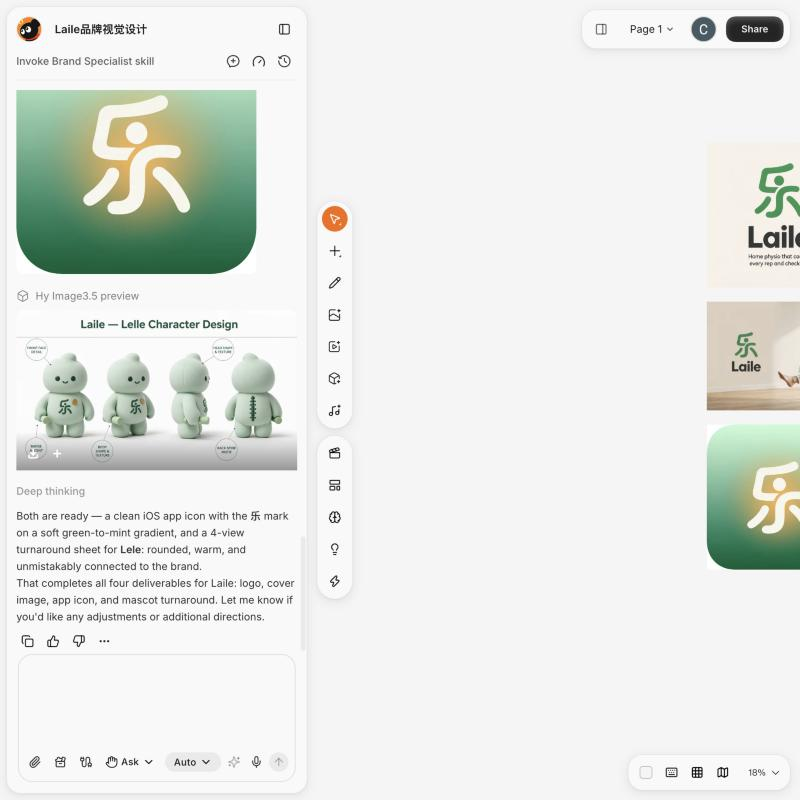
\includegraphics[width=0.47\linewidth]{../codebuddy/07-miora-brand-chat.jpg}}\hfill
\fbox{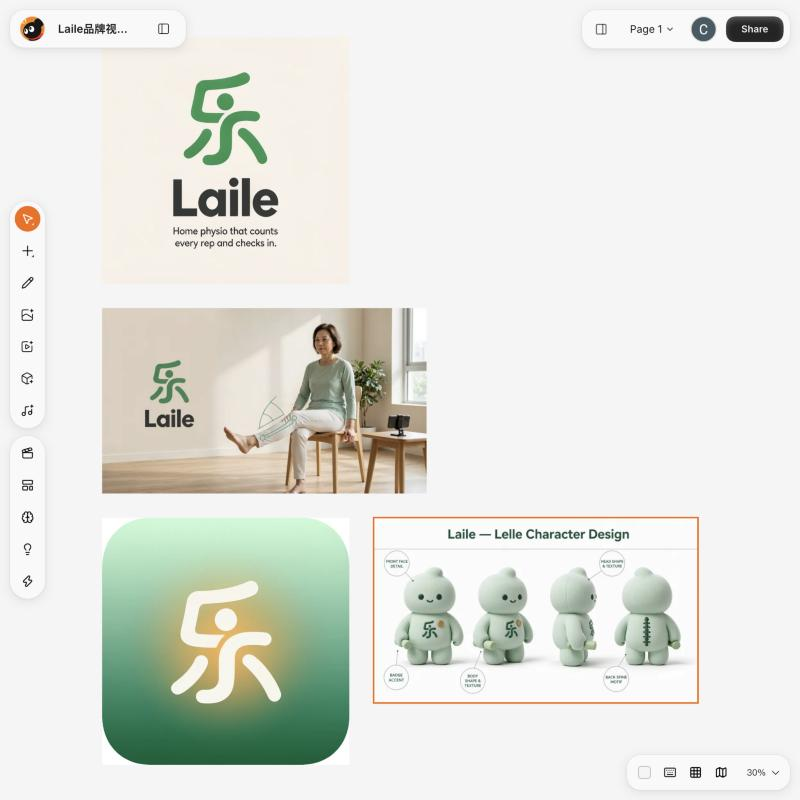
\includegraphics[width=0.47\linewidth]{../codebuddy/08-miora-brand-canvas.jpg}}
\caption{The Laile brand project in Miora: the conversation that produced the app icon and mascot (left) and the four deliverables on its canvas (right).}
\end{figure}

\subsection*{Audited and fixed with CodeBuddy}
In the final week the code was handed to WorkBuddy, CodeBuddy's coding agent (Tencent Hy4 model), through its GitHub connector. It cloned the repository, ported the safety rules to Python to test real phrasings against them, and later installed a Swift toolchain to compile and run its own changes. Three tasks:
\begin{itemize}
  \item \textbf{Safety audit} of the symptom rules. Findings included: a denial of pain hid numbness (``no pain but my foot is numb'' was answered with ``carry on''); denials raised false emergencies (``no chest pain'' told the person to call 995); a red flag judged by the model could never reach the emergency level; the server's pain threshold could become 11 on a 0 to 10 scale; a stop decision during rest was ignored; and common wordings were missed (``my chest is really tight'', ``my incision is leaking'', falls).
  \item \textbf{Safety fixes.} WorkBuddy implemented all six fixes with tests for every case in its audit; 112 core tests passed in its own Swift toolchain (92 before). The commit was reviewed and merged under CodeBuddy's name, followed by a review commit that keeps ordinary workout talk (``my heart is racing'', ``I fell asleep'') from raising red flags.
  \item \textbf{ADP and reply review.} Sixteen findings on the Lele integration, the most serious being that ``I haven't taken it yet'' was logged as a taken medicine dose, plus reasoning text that could leak into replies, no server-side timeout on the ADP call, and a failed turn that could not be retried. The confirmed findings were fixed with regression tests: reminder answers now need a clear ``taken'', negated answers (``no more pain'') no longer save a flare, only reply messages reach the person, and outbound calls time out.
\end{itemize}

\begin{figure}[htbp]
\centering
\fbox{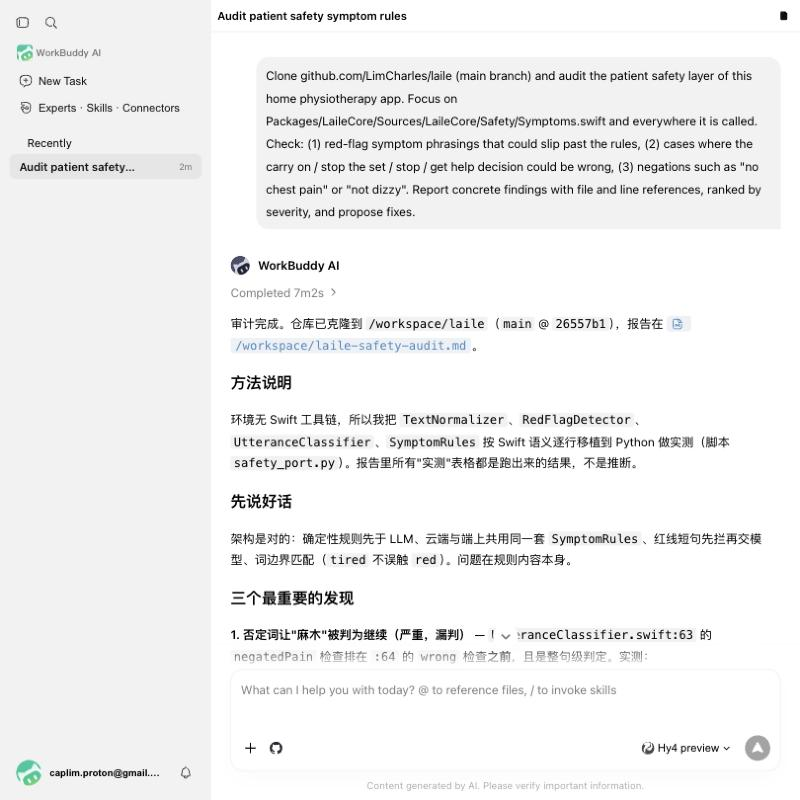
\includegraphics[width=0.47\linewidth]{../codebuddy/01-safety-audit-request.jpg}}\hfill
\fbox{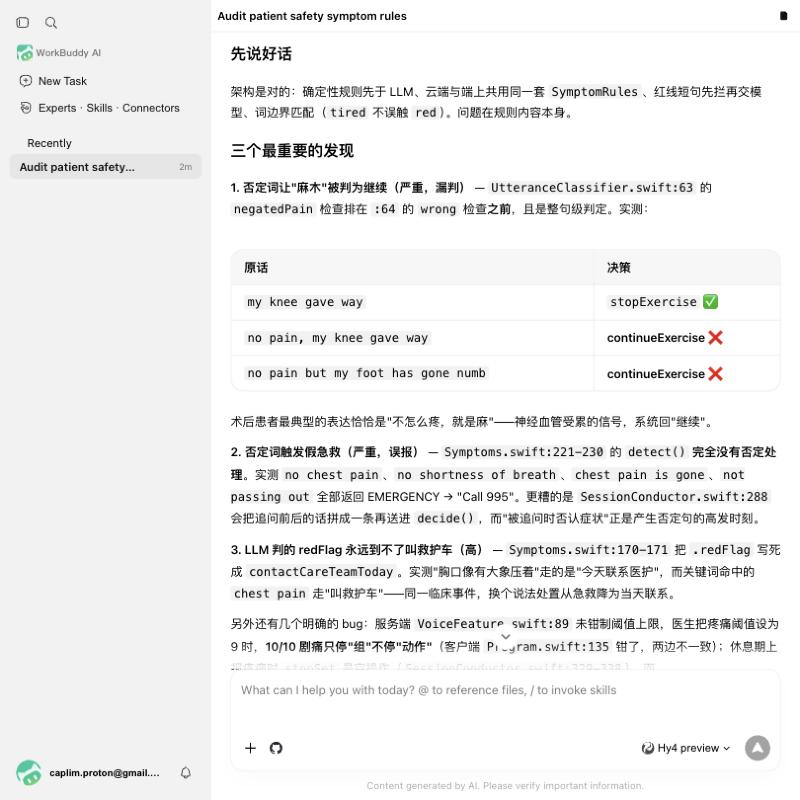
\includegraphics[width=0.47\linewidth]{../codebuddy/02-safety-audit-findings.jpg}}\\[6pt]
\fbox{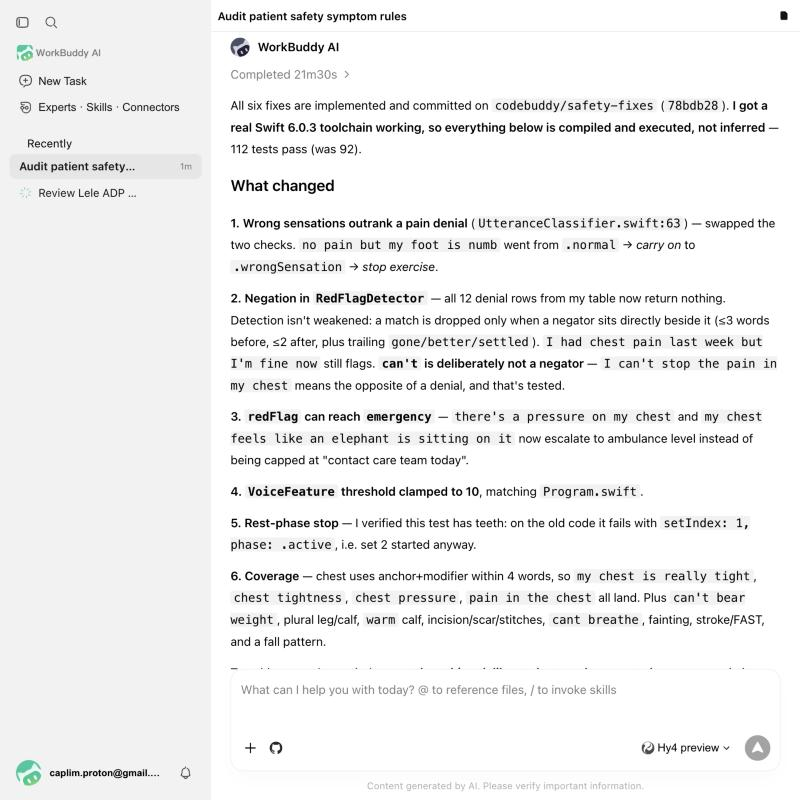
\includegraphics[width=0.47\linewidth]{../codebuddy/06-safety-fixes-done.jpg}}\hfill
\fbox{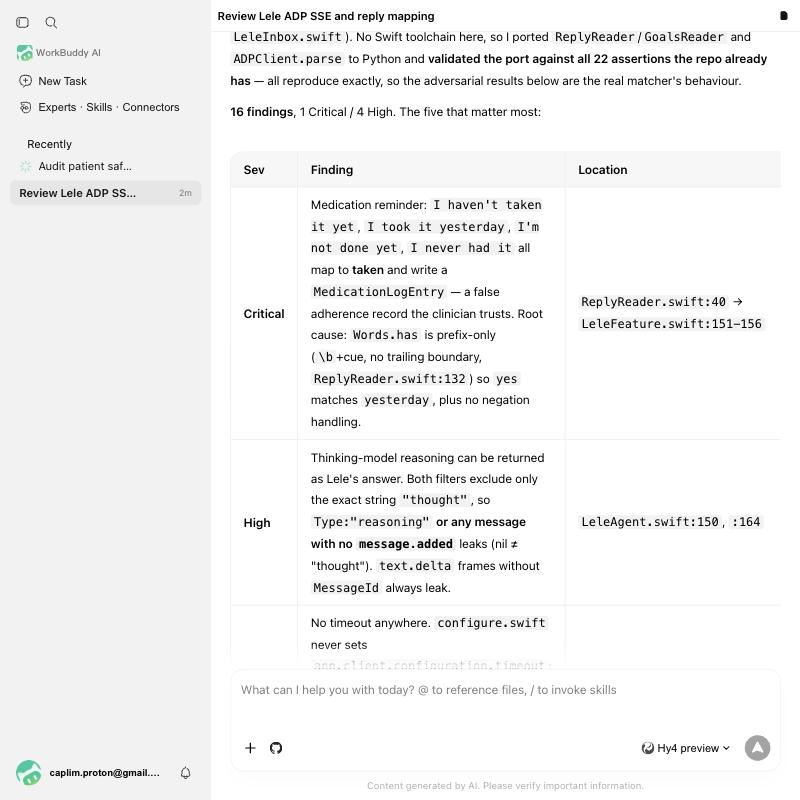
\includegraphics[width=0.47\linewidth]{../codebuddy/05-adp-review-findings.jpg}}
\caption{WorkBuddy (CodeBuddy) sessions on the Laile repository: the safety audit request and its findings (top), the implemented safety fixes and the ADP integration review (bottom).}
\end{figure}

\begin{thebibliography}{9}\small
\bibitem{argent2018} Argent R, Daly A, Caulfield B. Patient involvement with home-based exercise programs: can connected health interventions influence adherence? \emph{JMIR mHealth and uHealth}. 2018;6(3):e47. \url{https://mhealth.jmir.org/2018/3/e47/}
\bibitem{jack2010} Jack K, McLean SM, Moffett JK, Gardiner E. Barriers to treatment adherence in physiotherapy outpatient clinics: a systematic review. \emph{Manual Therapy}. 2010;15(3):220-228. \url{https://shura.shu.ac.uk/5146/}
\bibitem{peek2016} Peek K, Sanson-Fisher R, Mackenzie L, Carey M. Interventions to aid patient adherence to physiotherapist prescribed self-management strategies: a systematic review. \emph{Physiotherapy}. 2016;102(2):127-135. \url{https://doi.org/10.1016/j.physio.2015.10.003}
\bibitem{nptd2026} National Population and Talent Division, Strategy Group, Prime Minister's Office. \emph{Population in Brief 2026}. Singapore; September 2026.
\end{thebibliography}

\end{document}
